%!TEX root = ../thesis.tex
\mychapter{Implementation}{Implementation}{}
\label{chap:implementation}
\tikzset{
  blk/.style={draw, rounded corners=2pt, align=center, font=\footnotesize,
              minimum width=2.6cm, minimum height=0.95cm, inner sep=3pt},
  mdl/.style={blk, fill=black!8},
  hw/.style={blk, dashed},
  st/.style={draw, rounded corners=2pt, align=center, font=\footnotesize,
             minimum width=2.7cm, minimum height=0.9cm},
  arr/.style={-{Stealth[length=2mm]}, thick},
  lbl/.style={font=\scriptsize, fill=white, inner sep=1pt}
}


In the design chapter (Chapter~\ref{chap:design}), we went over what each pat of the pipeline does at a higher level. The following chapter
says how each of these part is actually built: the libraries, the process, layout, the message formats and how design decisions were turned instrumentation
code. There re no specific numbers references in the design chapter. The implementation chapter is where values are defined and implemented.

\mysubsection{Speech input and output}{Speech Input and Output}
\label{sec:speech}

All the audio files are transcibed using \texttt{faster-whisper}, which is a CTranslate2 reimplementation of Whisper,
using the \texttt{digiphyte/\allowbreak fluister-turbo} model. The model was chosen over a stock Whisper model because it is transcibed
to include South African English and Afrikans accents. That is important since I have a South African English accent. The model runs on the CPU
with \texttt{compute\_type="int8"} and 8 threads. The reason for not running it off the GPU is to save on VRAM which can be used for the planner and
vision models. Since the audio clips are short enough that the CPU does not become the bottleneck when transcribing the audio.

Audio arriving as an encoded container (webm/mp4/wav) and is decoded to a 16kHz mono PCM waveform via FFmpeg, which is a a multimedia library before being passed to the Whisper 
encoder. The raw samples are captured directly via sounddevice and can bypass this step.
The \texttt{transcibe\_audio} function takes either a raw bytes (which is an encoded clip form the turboPi, and decoded using FFmpeg) or using a Numpy array
of raw float samples. This function is called once per audio clip and not continueally as a audio streams in. This is because the rover does not have to continueally
listen to its surroundings for feedback. The audio clip is padded to 30\,s internally. Therefore to redunce the number of chunnks you would take on the audio clip.


\begin{figure}[htbp]
  \centering
  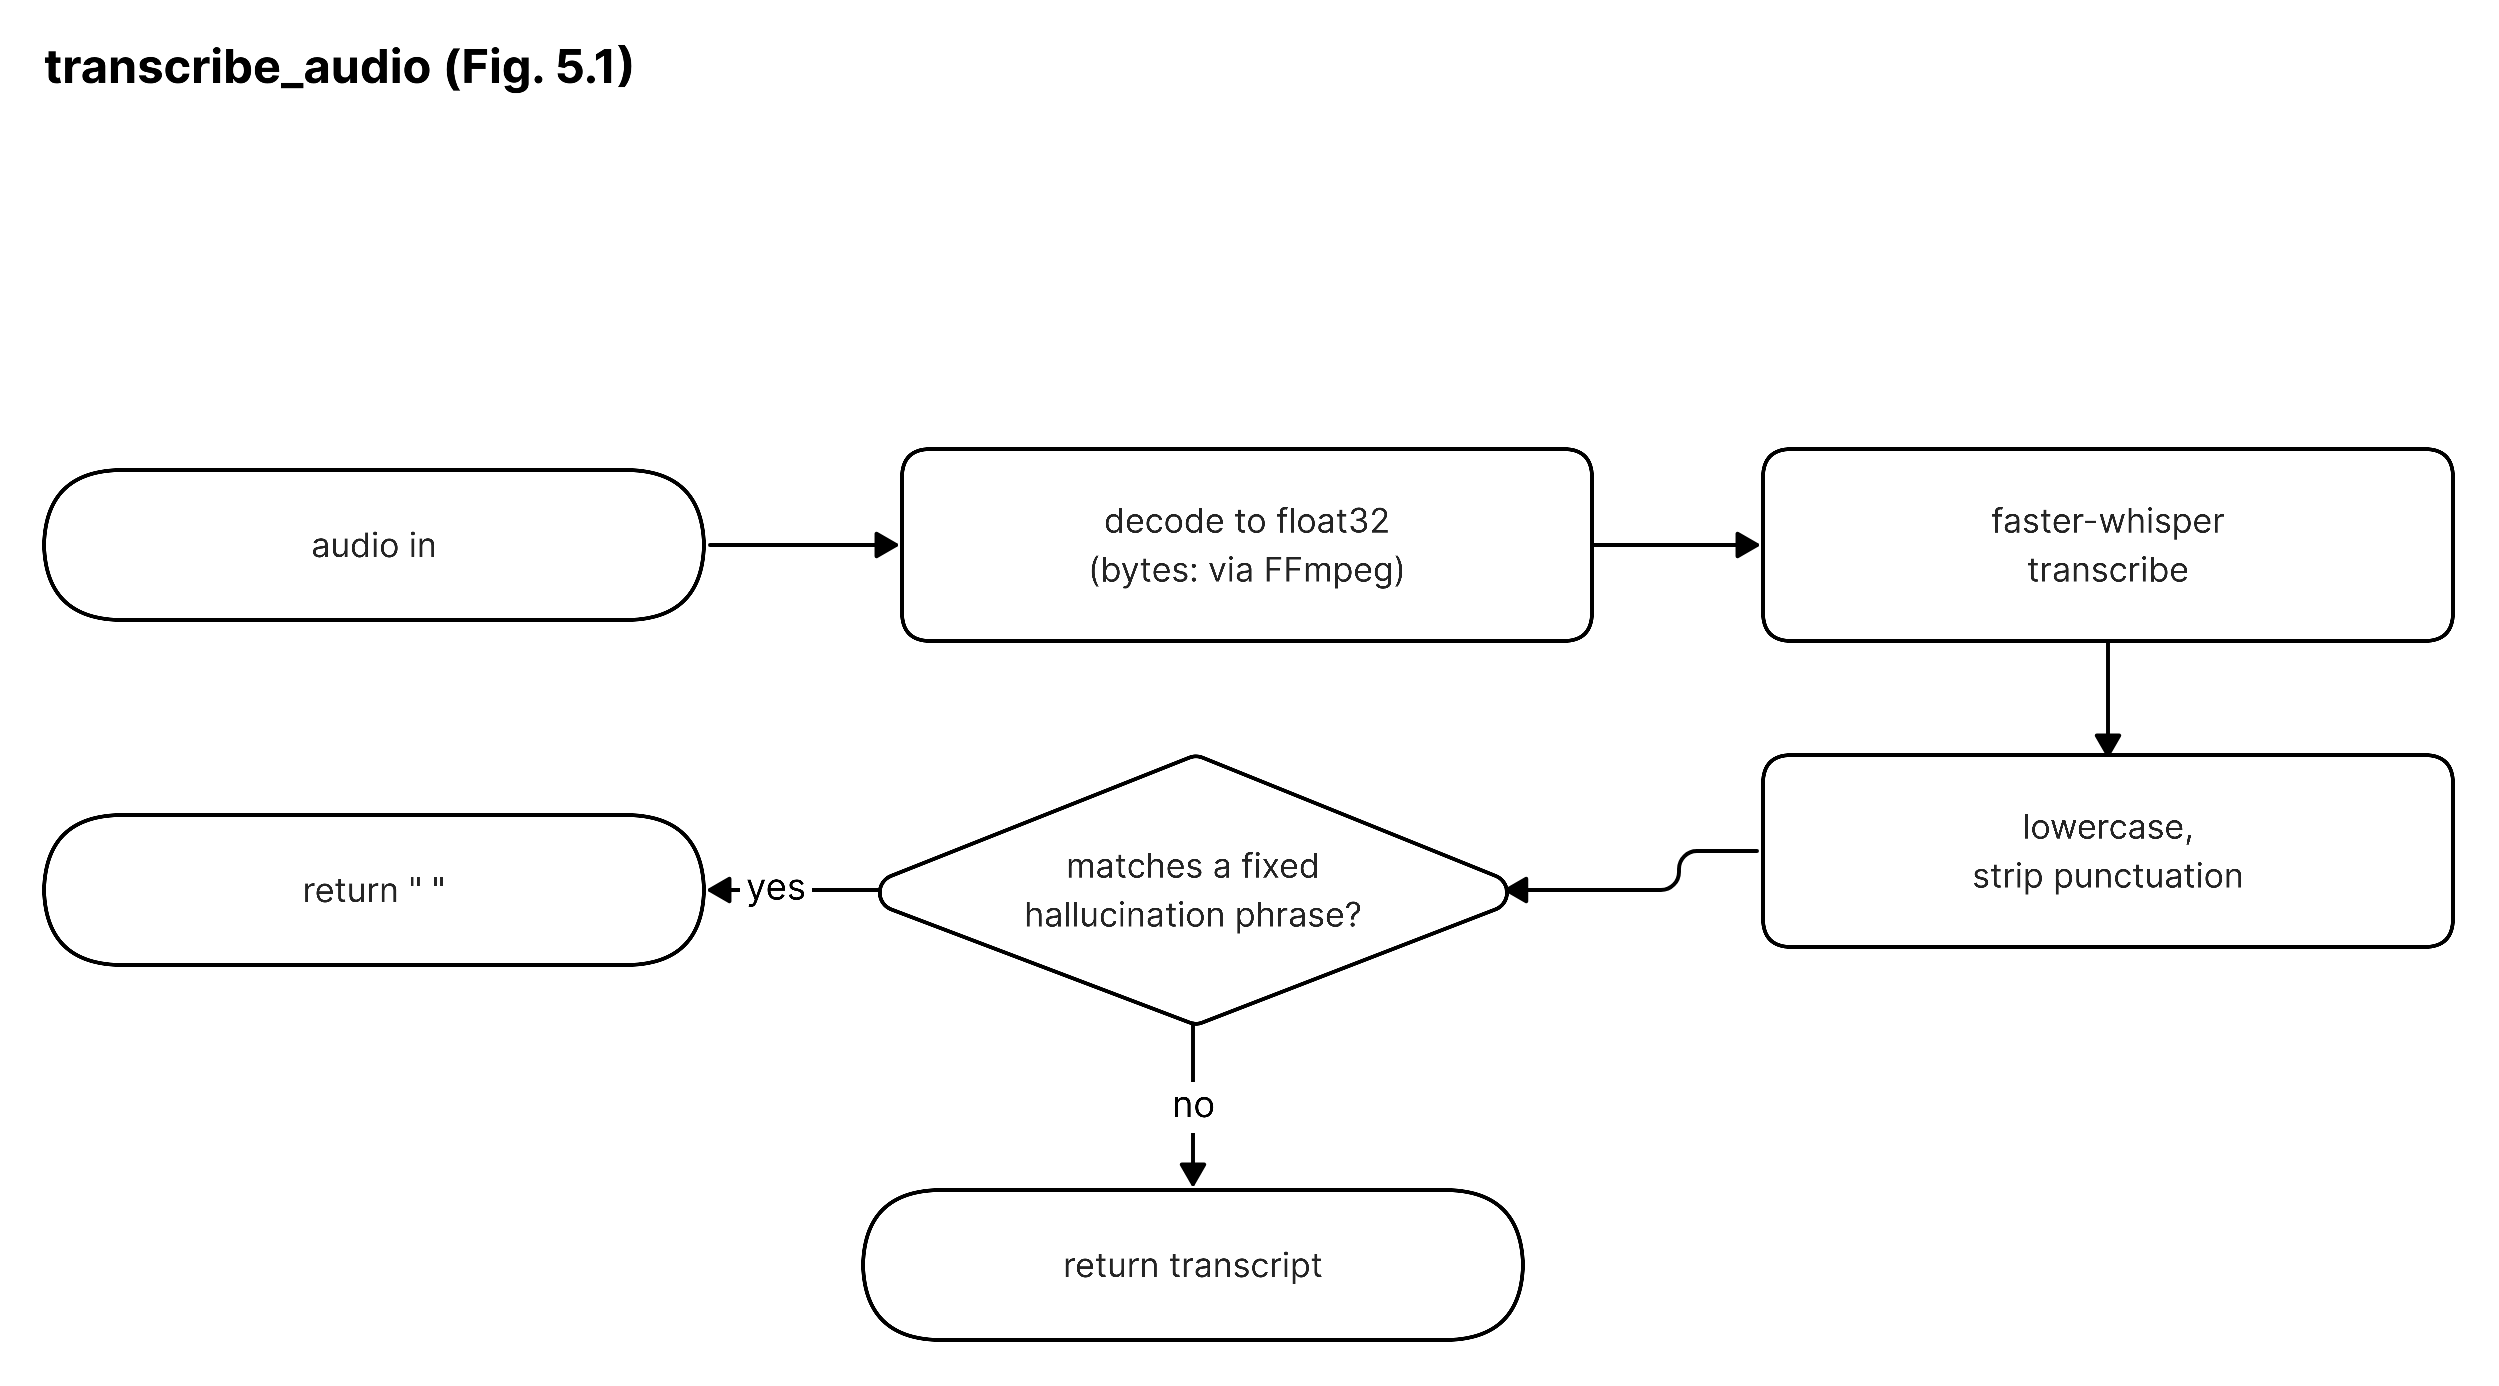
\includegraphics[width=\linewidth]{figures/fig5_1_flow_stt.png}
  \caption{\texttt{transcribe\_audio}. The hallucination check exists because \texttt{fluister-turbo} occasionally transcribes silence or background noise as one of a handful of fixed captioning artefacts, most often ``thank you so much for watching''.}
  \label{fig:flow-stt}
\end{figure}

A empty string is returned in place of all the phrases that are deemed to be hallucinations. It is treated as a failed command
rather than letting the planner model fail acting on a hallucination.

\mysubsection{Speech output: Piper}{Speech Output}
\label{ssec:tts}

For someone to actually hear the rover speak back. This goes through Piper, a local neural text to speech engine. which uses a 
\texttt{een\_US-lessac-medium} voice. The \texttt{tts.py} mirrors \textt{stt.py}'s way of caching-model pattern: \texttt{get\_voice}
will load the PiperVoice model once and keep it as a callable instance. Piper's voices are not fetched automatically the same way \texttt{faster-whipers}'s
model is. Initially I had to download the voice using: \texttt{python -m piper.\allowbreak download\_voices
en\_US-\allowbreak lessac-medium}. Then point the environment variable at the \texttt{.onnx} file as well as its \texttt{.onnx.json} config file. There is no 
Afrikaanse voice available so the models were only configured in english. 

\begin{figure}[htbp]
  \centering
  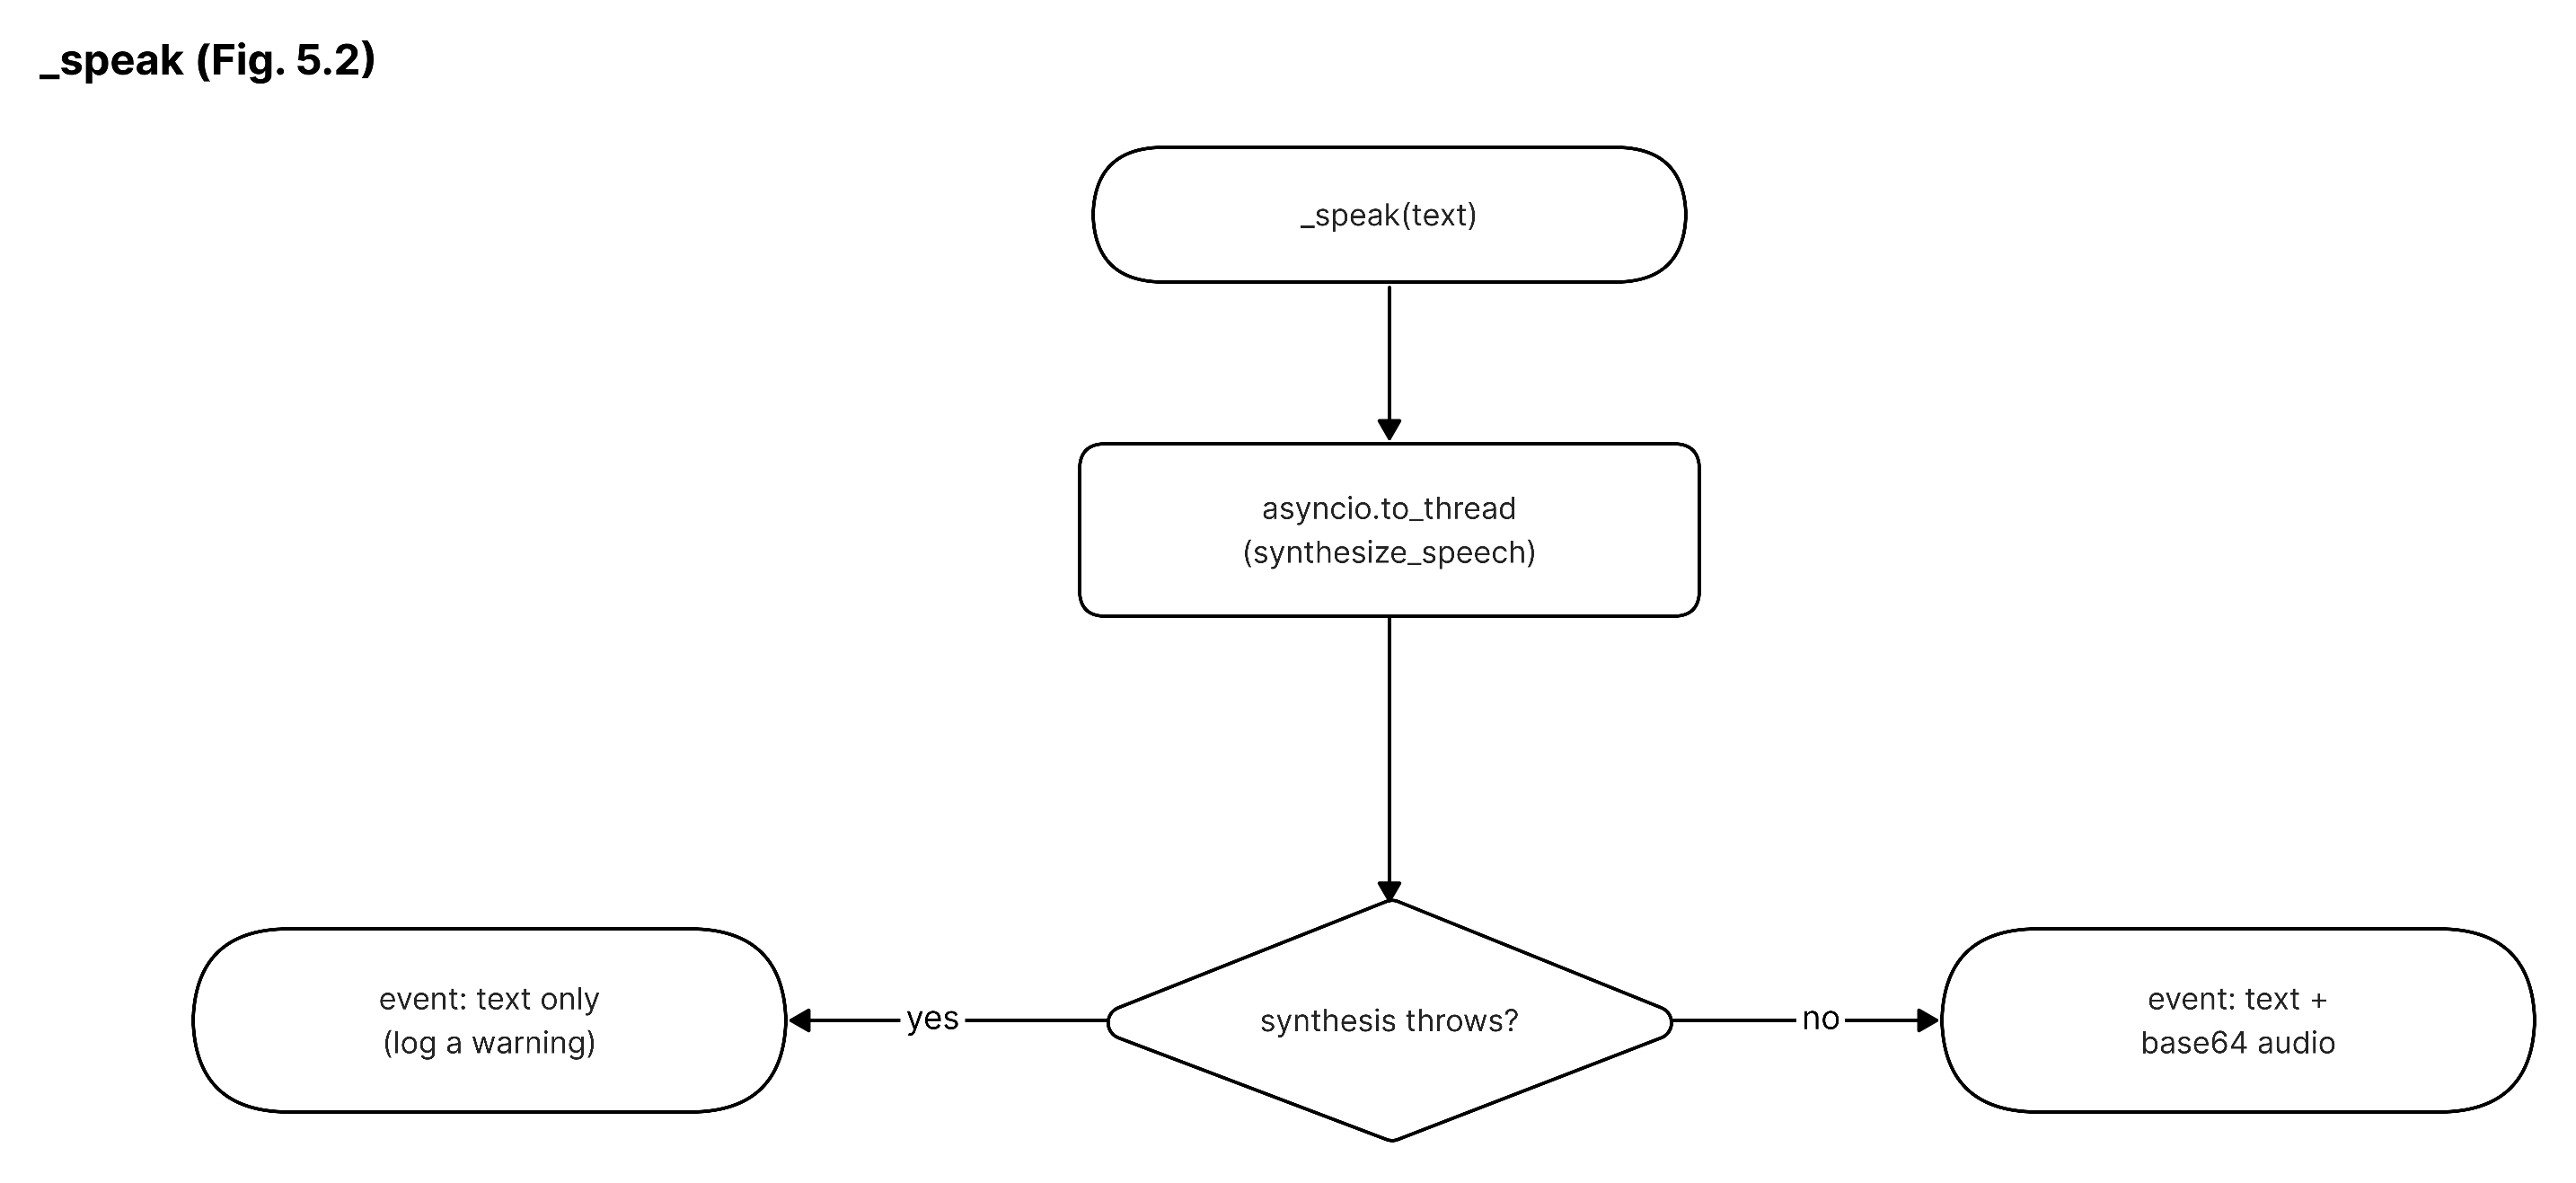
\includegraphics[width=\linewidth]{figures/fig5_2_flow_tts.png}
  \caption{Synthesis runs on a worker thread because \texttt{\_speak} shares an event loop with \texttt{ingest\_frame}: synthesis is sub-second but still blocking, and perception should not stall mid-mission for a voice line. A failure degrades the mission to text-only rather than stopping it, the same soft-fail stance the pre-departure dialogue's own \texttt{\_speak} in \texttt{pipeline.py} takes.}
  \label{fig:flow-tts}
\end{figure}

\mysection{Model inference layer}{Model Inference Layer}
\label{sec:inference}

\mysubsection{Planner}{Planner}
\label{sec:planner}

There is a \texttt{InferenceProvider} file which is an abstract class with one method, \text{complete}. This method takes lists of chat messages which as disguised as 
prompts as well as a optional image parameter and returns a \texttt{Completion} which has the following output. The text, which model answered, the latency as well as tokens used
as well as the cost which is seen in the report. There are currently wo providers local and cloud models. The local provider is called \texttt{OllamaProvider} and the cloud provider called \texttt{OpenAICompatibleProvider}.
Both providers implemented the same Input and output method described above. It is used since it is easy to interchange between cloud and local models. 

Every provider creation is cached by (role, provider, model), so a planner can be reused instead of reconstructin it on every call. Swapping the planner or vision model is a matter of an 
environment variable (\texttt{PLANNER\_PROVIDER}, \texttt{VLM\_PROVIDER}), not a code change. This stays in-tune with my modular design so testing different local models comes with ease.



\begin{figure}[htbp]
  \centering
  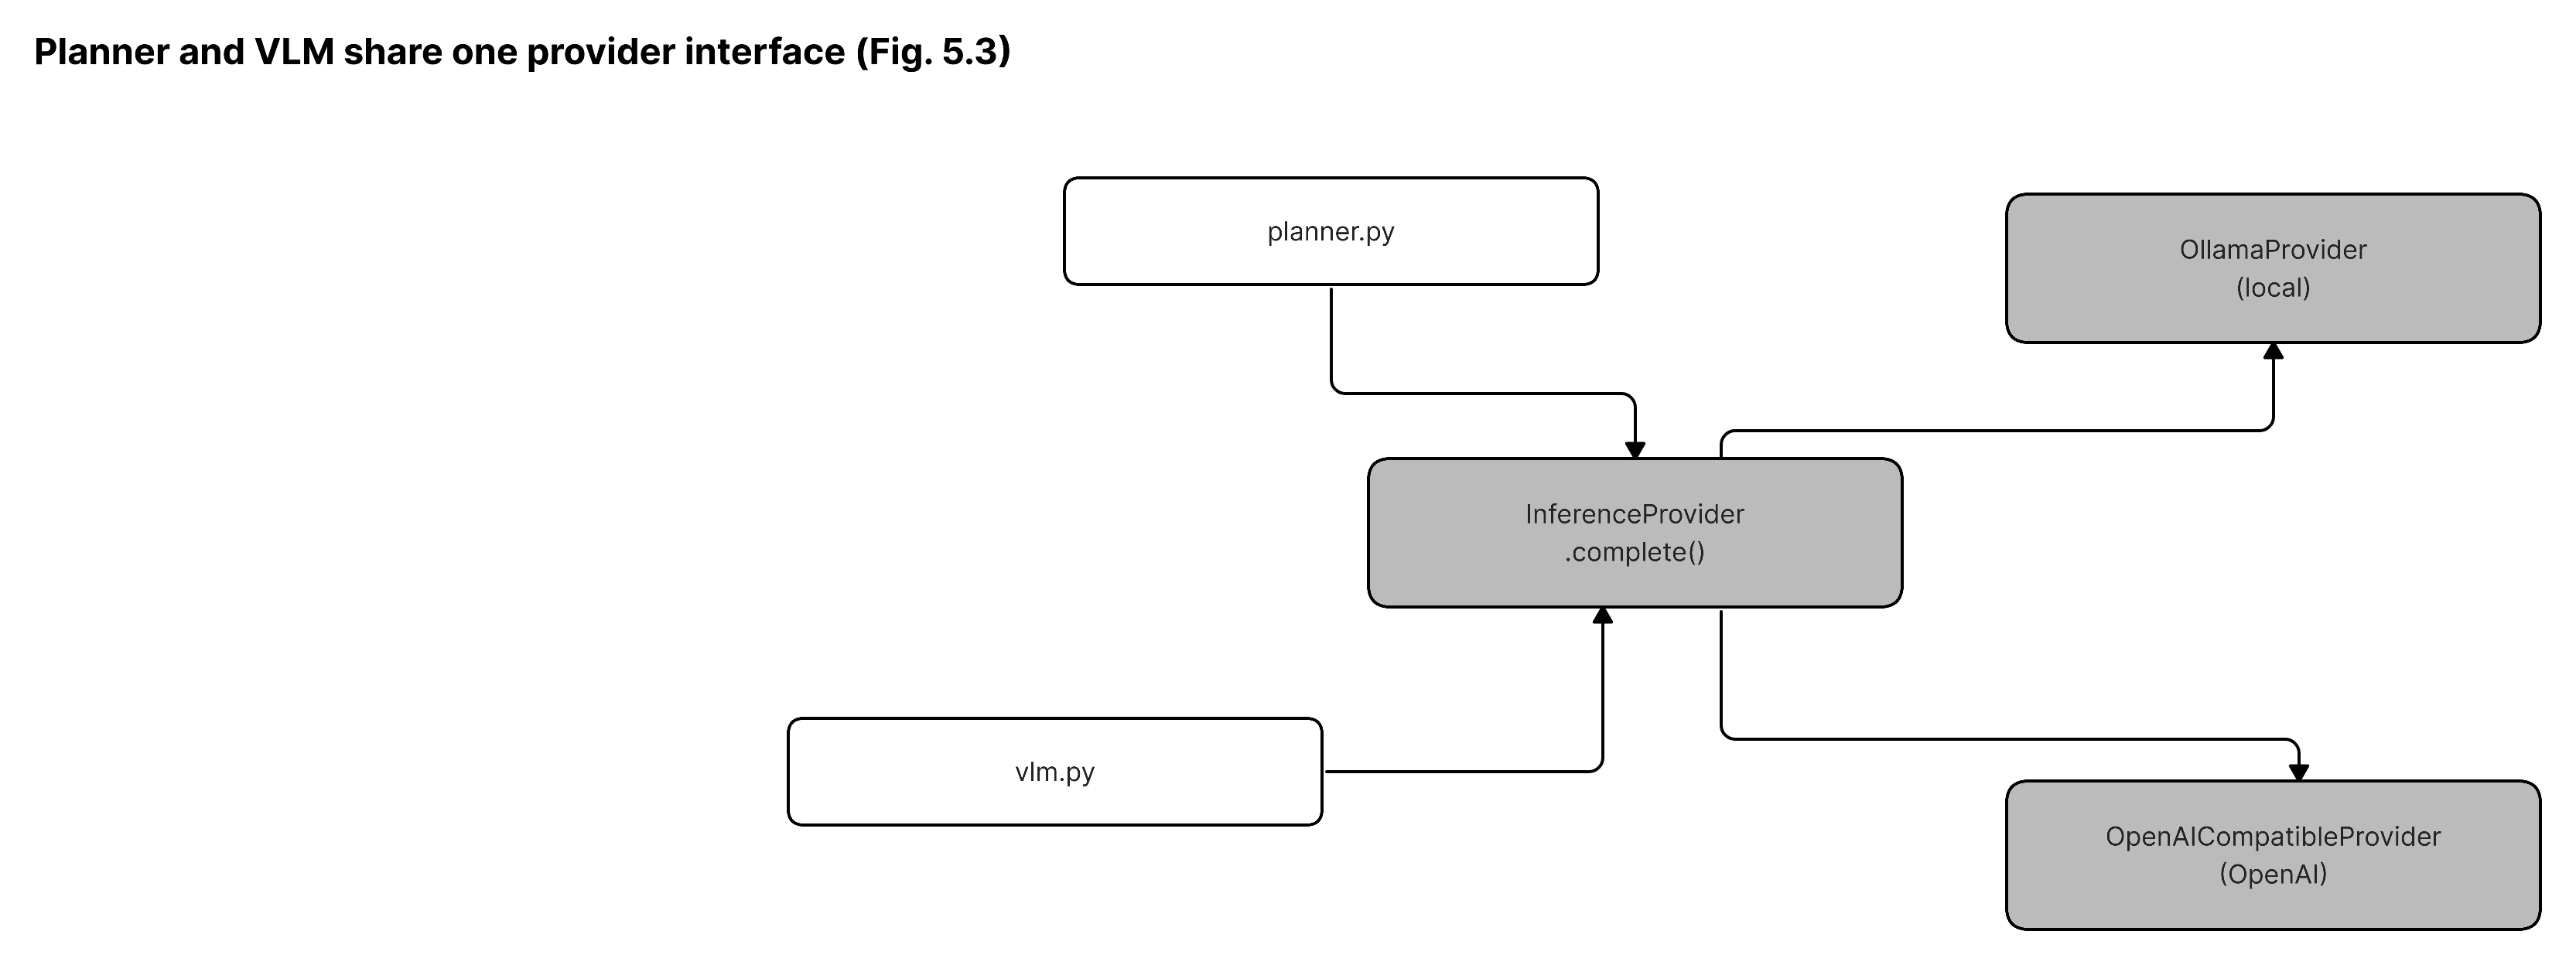
\includegraphics[width=\linewidth]{figures/fig5_3_providers.png}
  \caption{Both roles call the same interface. \texttt{get\_provider(role)} resolves \texttt{PLANNER\_PROVIDER} or \texttt{VLM\_PROVIDER} to a concrete class and caches the instance.}
  \label{fig:providers}
\end{figure}


The \texttt{OllamaProvideer} sends \texttt{num\_ctx} I defaulted this value to 8192 which I explain why in the Chapter~\ref{chap:evaluation}
An optional \texttt{repeat\_penalty} parameter is allowed, and \texttt{format="json"} for every planner and VLM call. Ollama allows you to call 
a model twice before it fails the missions. Two crashes which I ran into was a cold CUDA load on \texttt{gemma4:e4b} specifically and a small model loops on
the same tokens. \texttt{build\_plan\_prompt} function assembles a prompt form the active planner profile (Section~\ref{sec:vocabulary}), the room digest when 
one is loaded, and the conditioanl guidance block when the command contains a conditional word (Section~\ref{sec:condional}). A pure function which is seperate 
from \texttt{generate\_plan}. The following \texttt{tools/snapshot\_ptompt.py}, can print out the exact prompt a command would produce without calling a model.

\begin{figure}[htbp]
  \centering
  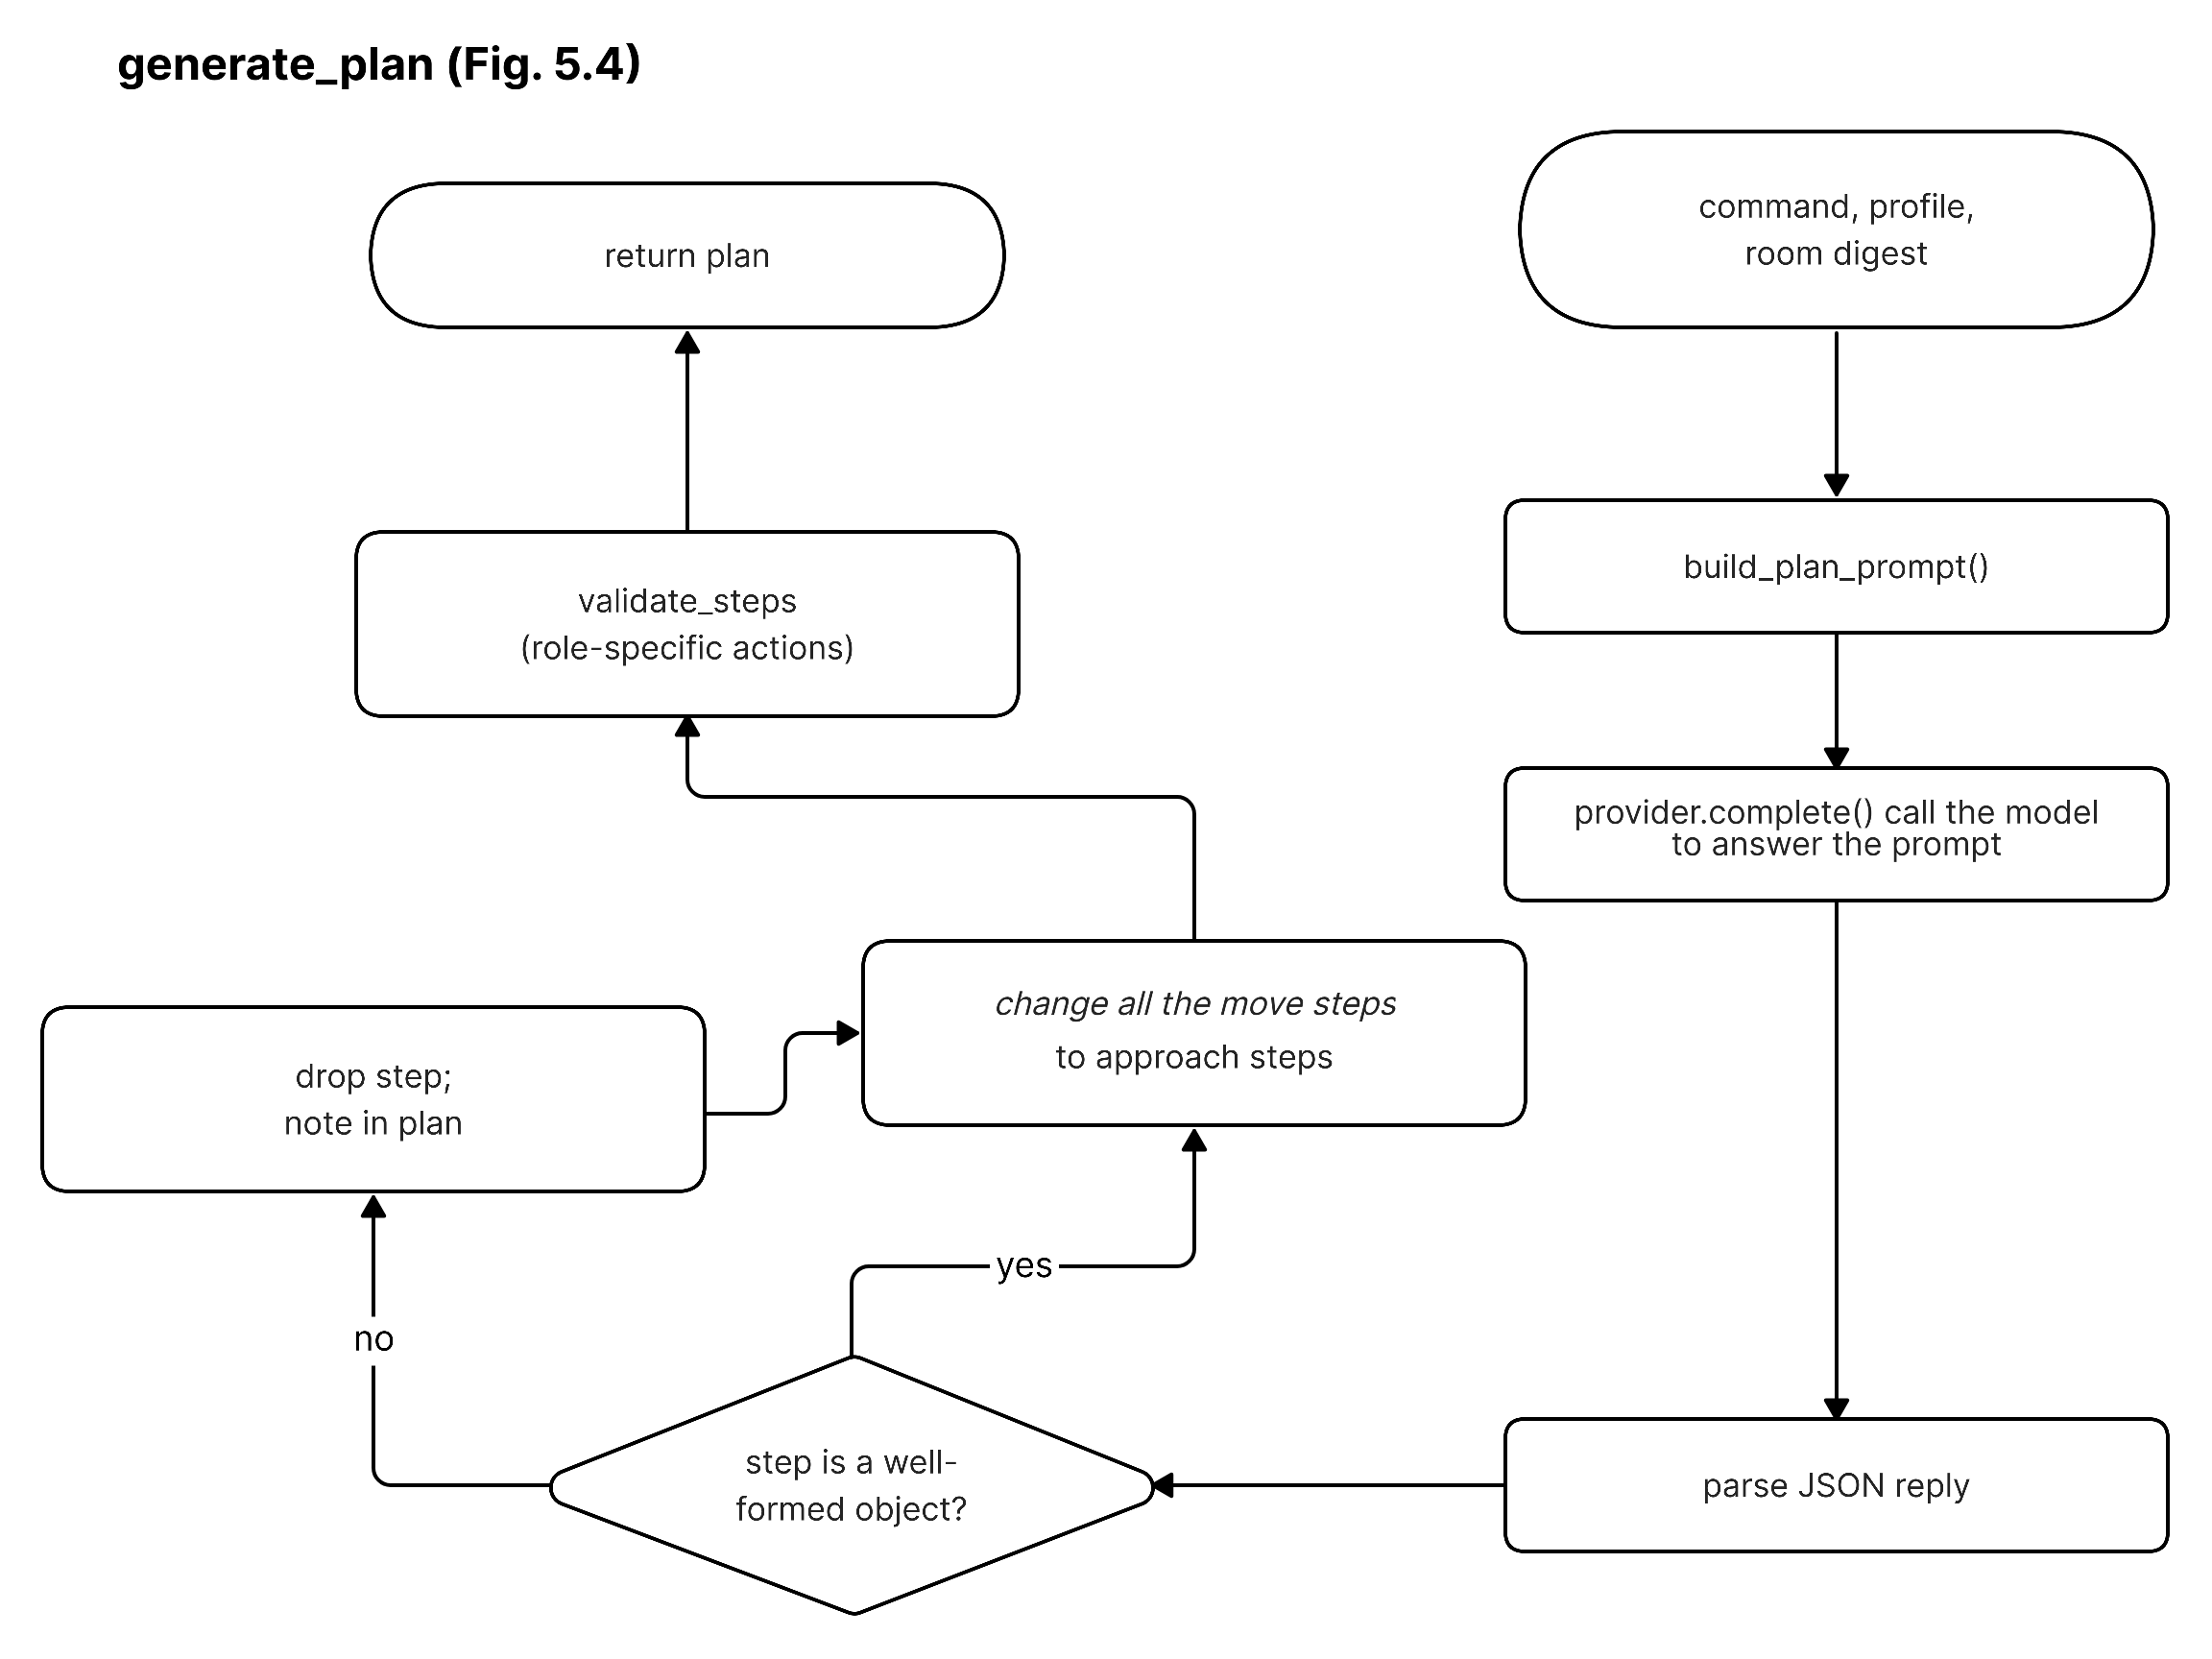
\includegraphics[width=\linewidth]{figures/fig5_4_flow_planner.png}
  \caption{\texttt{generate\_plan}. A smaller model sometimes writes a step as a bare string instead of an object, or nests the list oddly, so every step is checked before anything downstream calls \texttt{.get} on it. \texttt{\_promote\_moves\_to\_approach} rewrites a \texttt{move} step whose target names an object into an \texttt{approach} step (Section~\ref{sec:vocabulary}); the retried transient failures from \texttt{provider.complete()} are omitted here for space and described in the text above.}
  \label{fig:flow-planner}
\end{figure}

Having a look inside the Failure recovery (Section~\ref(ssec:guidance_loop)). There is an second prompt which is built using what 
we created called, \texttt{build\_replan\_prompt}, as well as a second ebntry point, \texttt{replan\_from\_state} used instead of 
using a parameter on \texttt{generate\_plan}. Since a replan is built from thee command as well s the steps which have been executed as
well as the steps which failed and why it failed. 

\mysubsection{Vision-language verification}{Vision-language Verification}
\label{sec:vlm}

All the calls which are made to a the local vision model go through one function, \texttt{\_ask}. This function takes a named stage,
a prompt, an optional image and a salvage flag. It then calls the correct VLM depending on the provider, cloud or local. Ollama also comes
with a parameter to set the output format to json using, \texttt{json\_mode=True}. Each previous function is a single shot prompt which then calls
the \texttt{\_ask} function to execute that step. The single purpose prompts are all functions namely: \texttt{check\_ambiguity}, \texttt{verify\_plan},
\texttt{describe\_frame}, \texttt{inventory\_frame}, \texttt{locate\_target},
\texttt{check\_condition} and \texttt{survey\_frame}. None of the prompts used follows a particular template as this can results in
the answer from the model having extra fields which are not intended.

\begin{figure}[htbp]
  \centering
  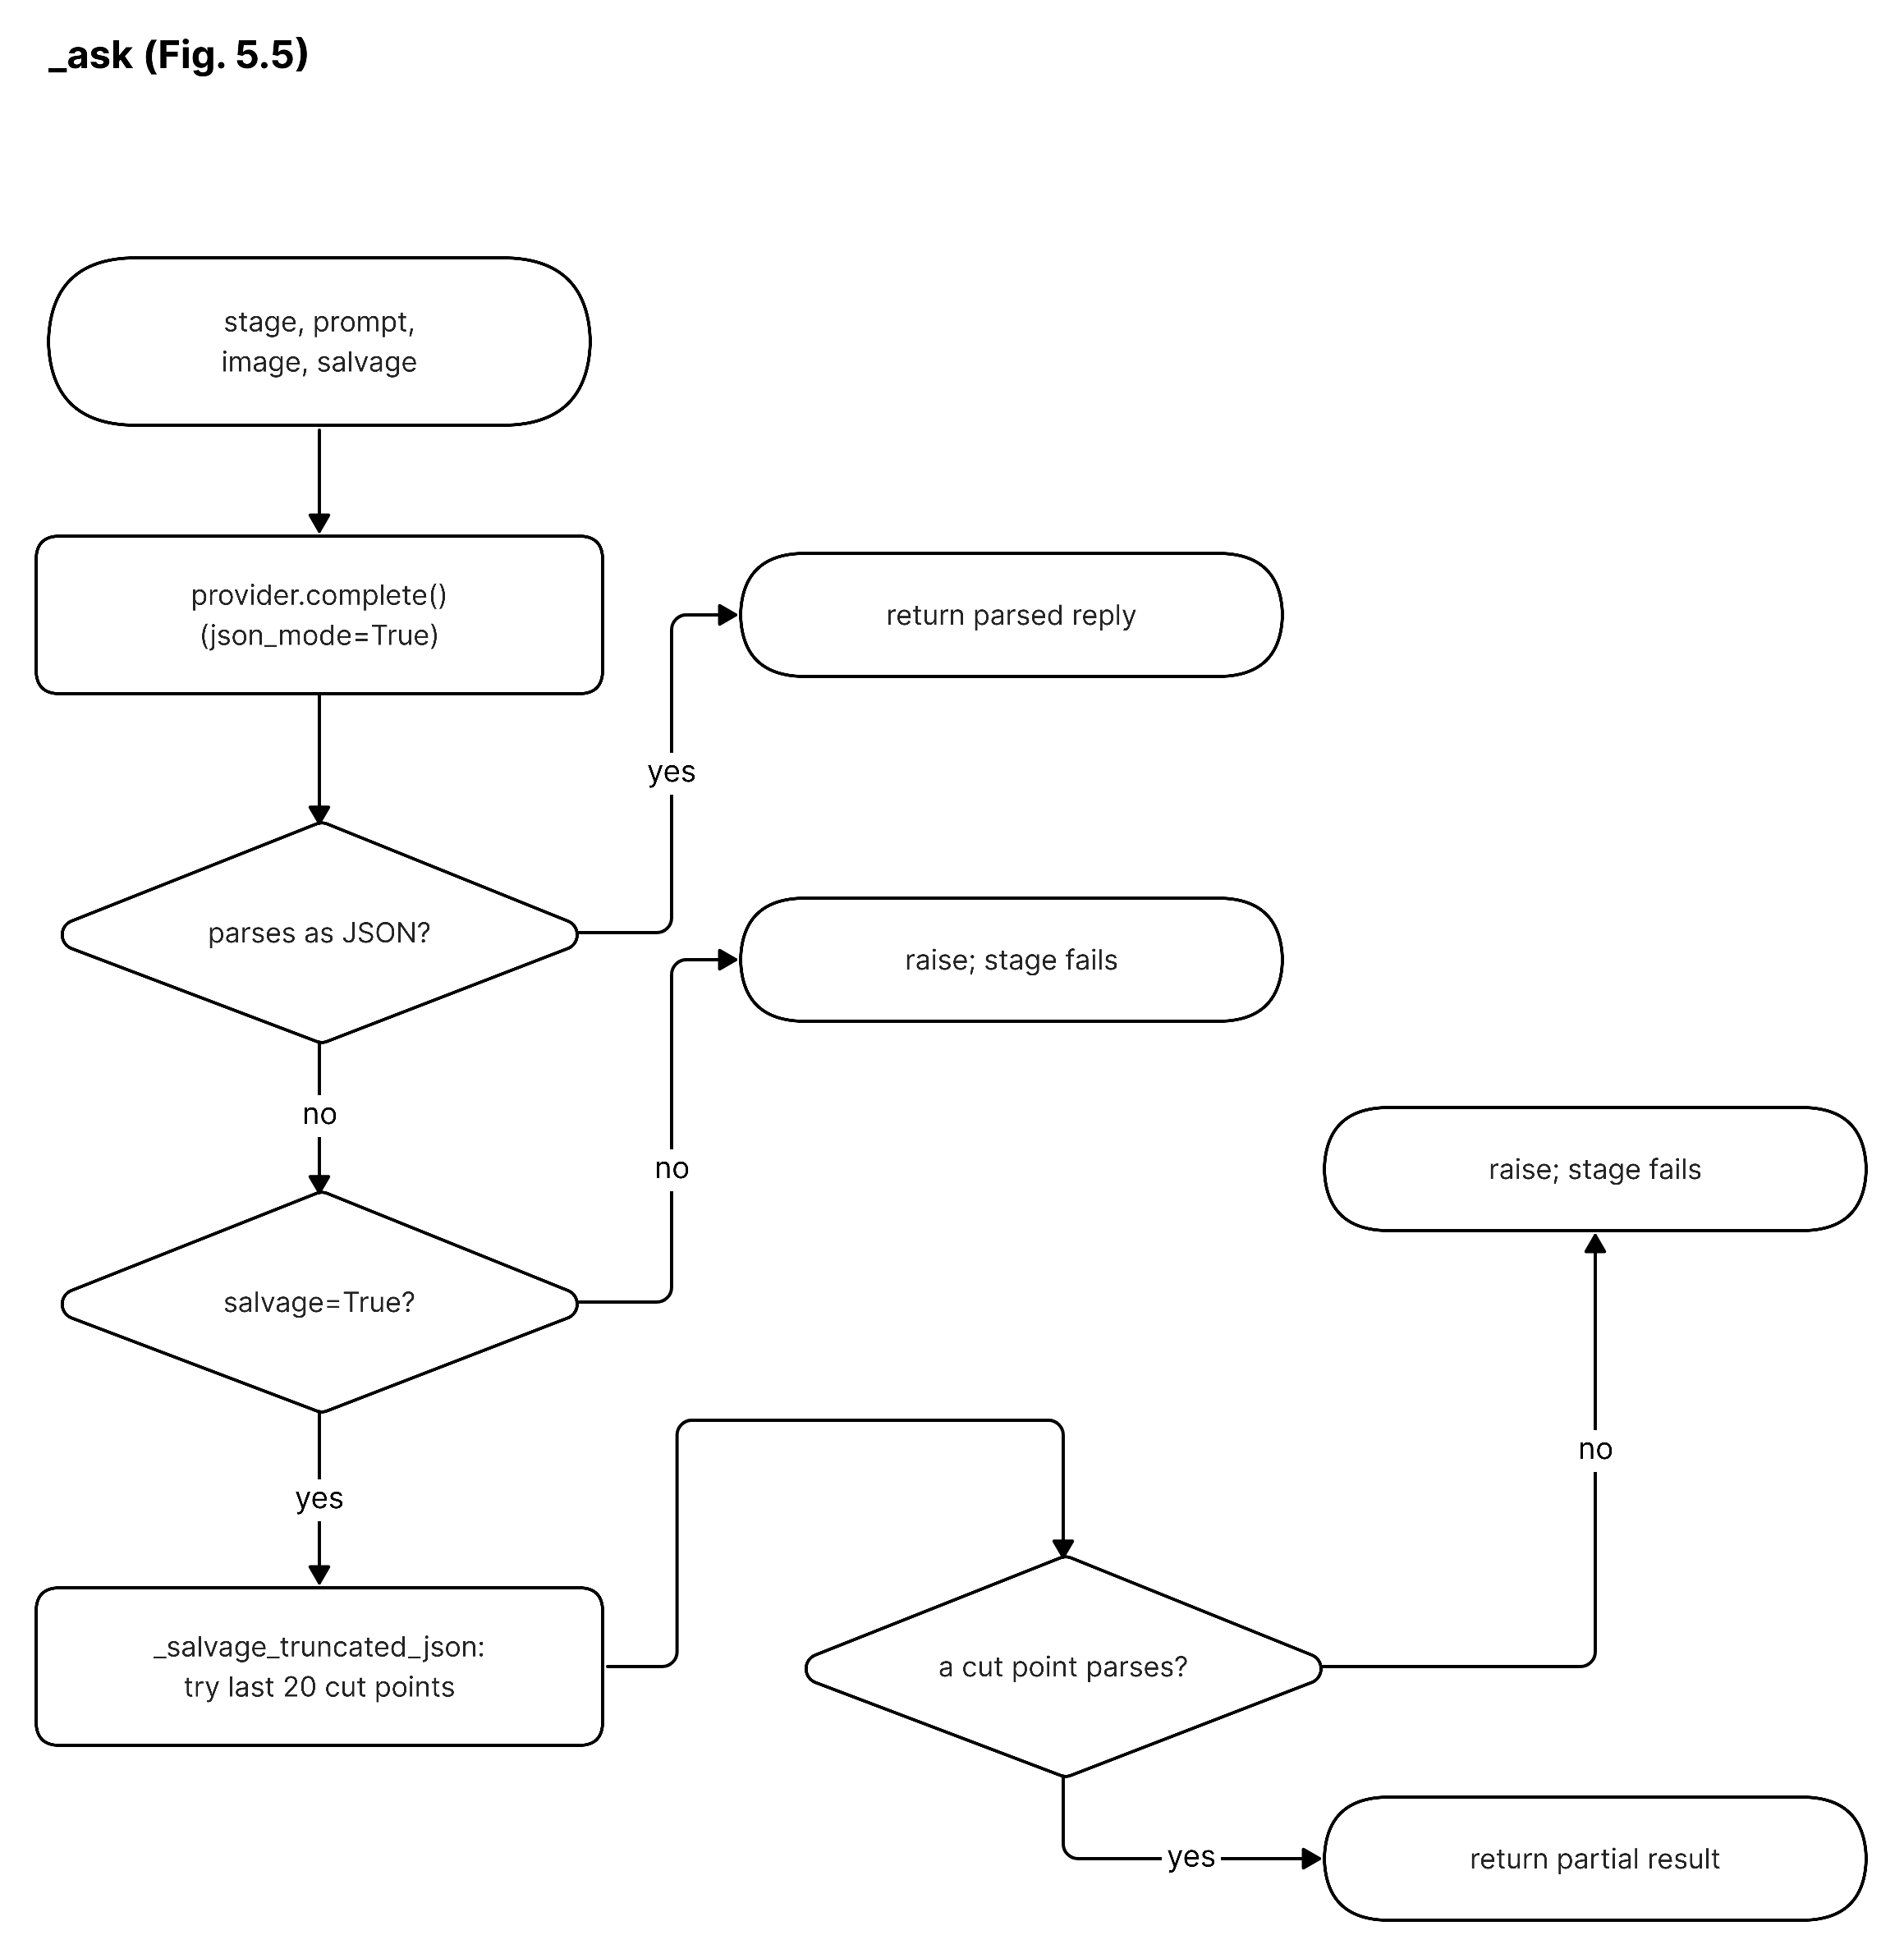
\includegraphics[width=\linewidth]{figures/fig5_5_flow_vlm.png}
  \caption{\texttt{\_ask}. Salvage is only enabled for \texttt{inventory\_frame} and \texttt{survey\_frame}, the two calls that ask for a list of objects and sometimes hit \texttt{num\_predict} mid-list on a model that has started repeating itself; a reply with ten correct objects and one truncated one is more useful than discarding it. Every other call keeps \texttt{salvage=False}, since a truncated yes/no answer or bounding box is not something a partial parse can safely recover.}
  \label{fig:flow-vlm}
\end{figure}


The \texttt{locate\_target} has the most moving parts. It is called once per cycle in the free-roam approach (Section~\ref{ssec:freeroam}).
The prompt asks the VLM for a bounding box, how confident it is in it's answer and how far away the object is. Using \texttt{distance\_cm\_from}
it converts whichever unit the model used inot centimetres, or if it fails it returns \texttt{None}. Any distance estimate that falls outside of
\((0,\;\texttt{VLM\_DIST\_MAX\_CM}]\), including a \texttt{NaN}, is also treated as if it were \texttt{None}. Any value that the model outputs is handled the 
same way. Since a model this small is small the predictions can be slightly incorrect

\mysection{Clarification and mission orchestration}{Clarification and Mission Orchestration}
\label{sec:orchestration}

\mysubsection{Clarificaiton manager}{Clarification Manager}
\label{sec:clarification_impl}

The clarification loop (Section~\ref{sec:clarification_design}) is a small state machine inside of ,\texttt{DialogueSession}, with
\texttt{Phase} as enumerator: (\texttt{CLARIFYING}, \texttt{PLANNING}, \texttt{VERIFYING},
\texttt{AWAITING\_CONFIRMATION}, \texttt{EXECUTING}, \texttt{REPORTING},
\texttt{CANCELLED}). There are also functions inside of \texttt{pipeline.py} which change the current Phase in which the rover is in.
This is built this way so that everyfunction inside of pipeline reads the phase before deciding what to do with incoming messages from the rover.
If boolean flags were used this would result in a state being missed or miss interepeted especially since most function calls inside the mission files make use of
worker threads.This would result in flags being set errouneously.


\texttt{effective\_command} helps to remove all the noise in the raw logs. Now the reason for there is three checks for the command 
at different stages. The resolved command once the vision model has written one, the orginal command spoken if the dialogue sessions reaches
its cap and the current command with the dialgue after all the clarification questions. Using only 1 function to update the command resulted in
the dashboard, the planner and the logs always having the same updated command.



The confirmation file has a smaller state machine inside of \texttt{confirmation.py}, and this is seperated from the normal Dialogue session.
Since its only job is to turn whatever was said into a yes, no or unclear output. The \texttt{keyword\_pass} function checks the reply given again English and an
Afrikaans phrase list. The rejected list is check first so a phrase like 'no, don't go'. Is not classified as 'yes' to go. This part of the pipeline does not
need a model to interpret what it should do. Since either the rover should go, 'yes',  or It should stay, 'no'.

\begin{figure}[htbp]
  \centering
  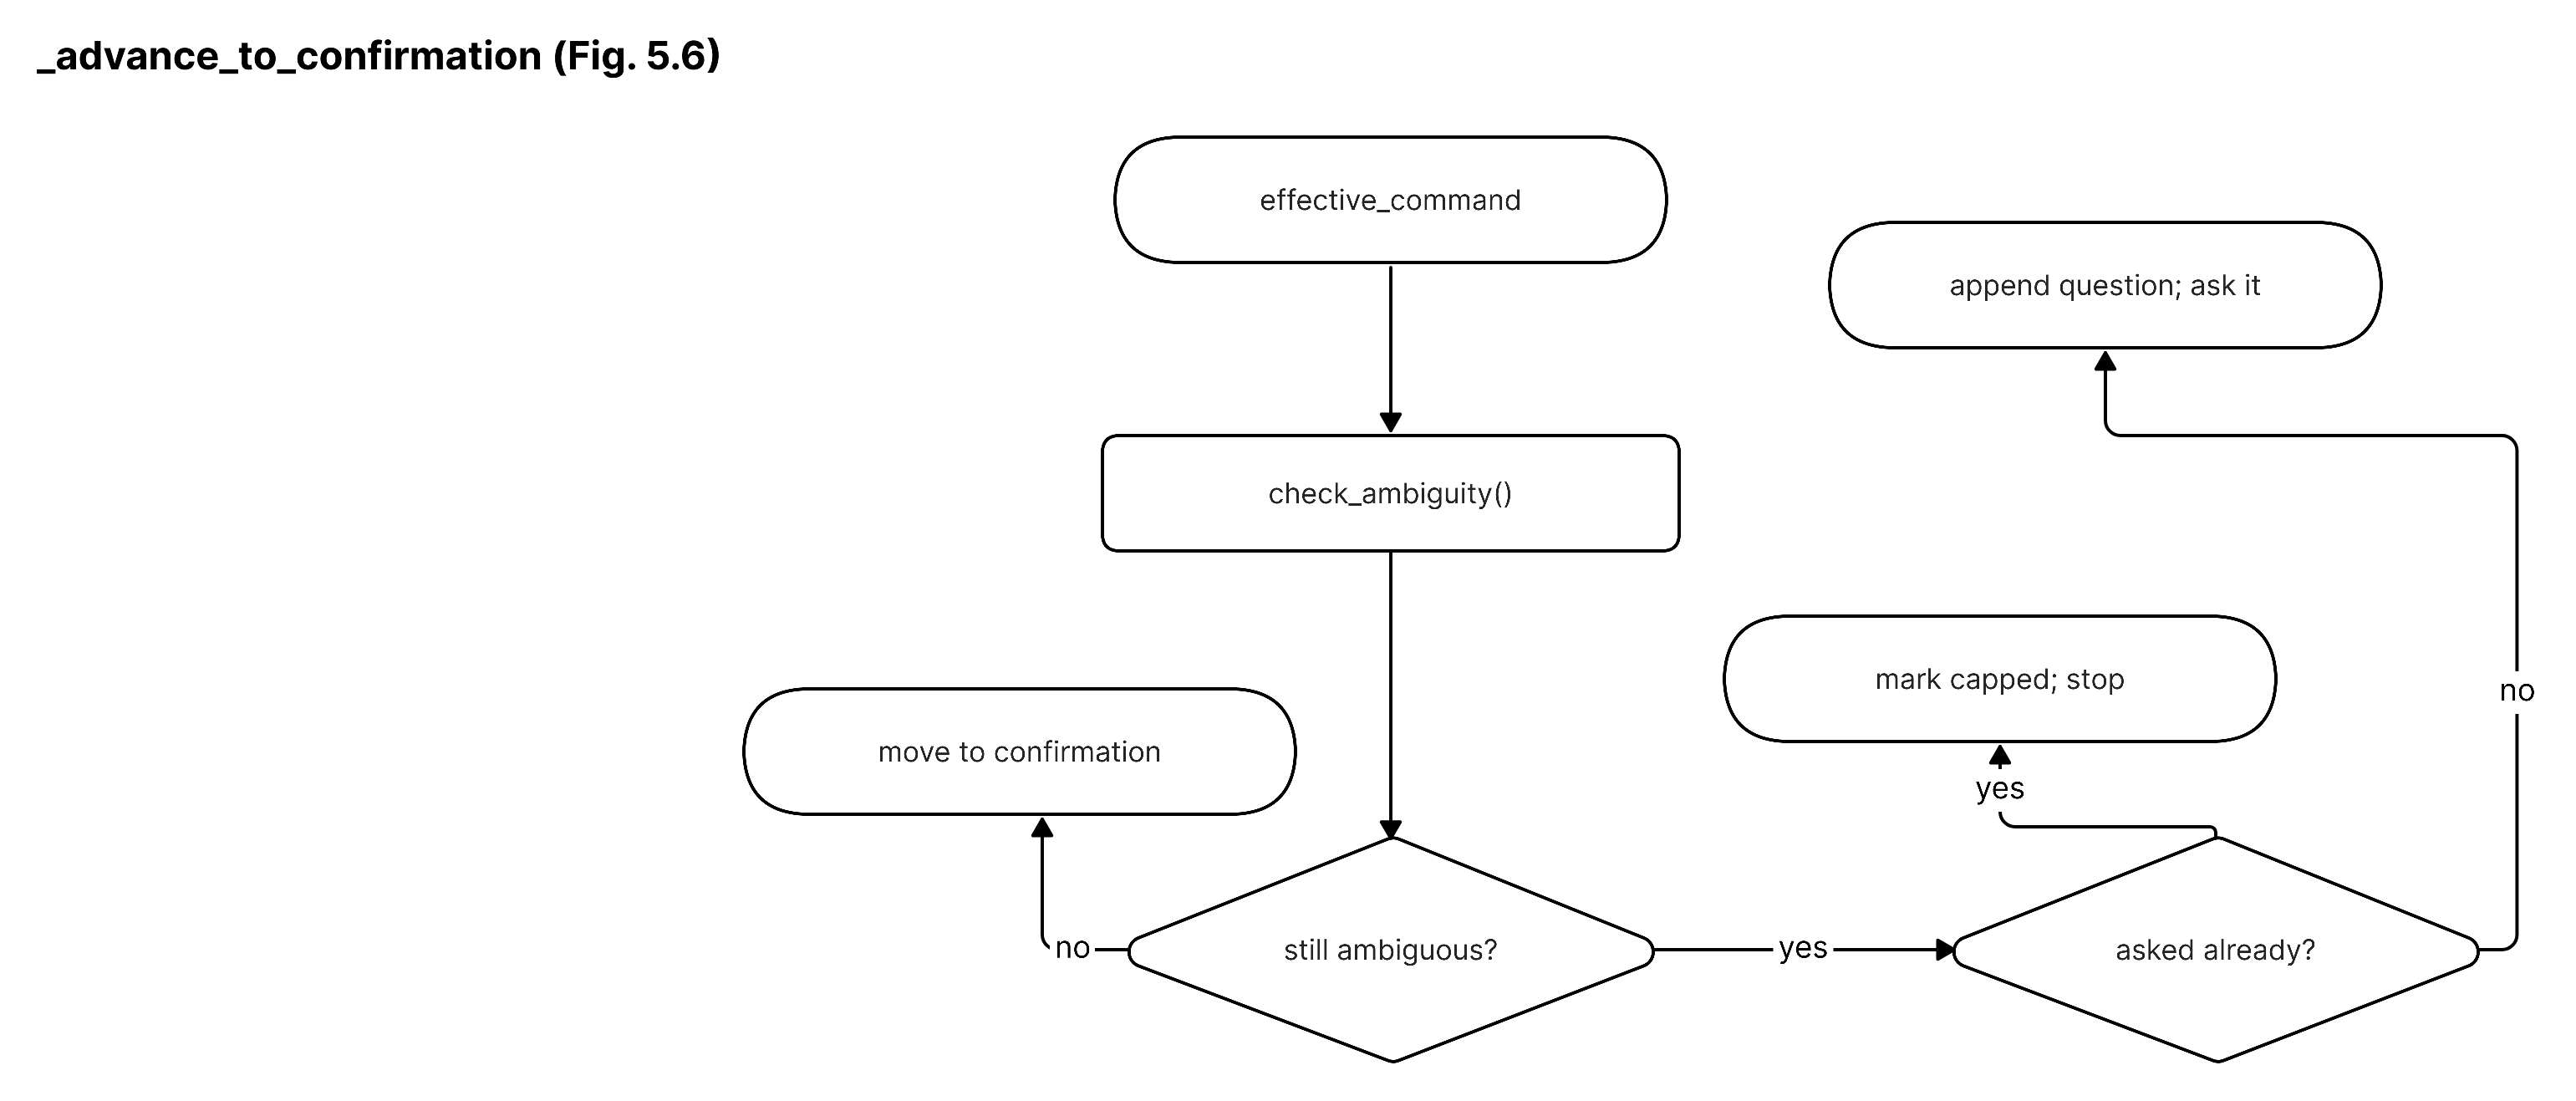
\includegraphics[width=\linewidth]{figures/fig5_6_flow_clarify.png}
  \caption{\texttt{\_advance\_to\_confirmation}, one turn of the clarification loop. The repeat-question check exists because a model that cannot think of anything new to ask would otherwise repeat the same question until the five-turn cap was reached, rather than giving up as soon as it had nothing left to add.}
  \label{fig:flow-clarify}
\end{figure}


Once the back and forth dialogue between the rover and the human is done. The \texttt{DialogueSession} 
hands the mission state off to \texttt{MissionSession}. Once that is complete the rover is no in a new state of
executing and will only communicate back to the user if it needs help with guidance or if it has arrived. The state
machine at play here is mission phases. 


\mysubsection{The mission execution loop}{The Mission Execution Loop}
\label{ssec:mission_loop}

Once the plan is confirmed, \texttt{run\_mission} is one function that drives the rover, one step at a time, 
until the mission reaches its terminal phase or it ran out of approach steps. This is kept as one function for
simplicty since if it was written in a class with multiple methods it would complicate it more. It does 4 things in
a loop. Read the cursor, run one step, decide what the results mean and move to the next step. If it was written in a 
class it would mean passing in the arguements between different methods and that would be more debugging work.

Which function actually runs a step depends on what the step is and on
what the rover object in use can actually do, and that second condition
matters just as much as the first. A \texttt{check} step goes to
\texttt{\_run\_check}. An \texttt{approach} step goes to
\texttt{approach\_controller} (the free-roam hop loop,
Section~\ref{ssec:freeroam}), but only when \texttt{NAV\_MODE} is
\texttt{free} and the rover object exposes \texttt{pivot}, \texttt{hop},
\texttt{get\_frame} and \texttt{set\_gimbal}. Everything else, including
every \texttt{approach} step when free roam is off, goes straight to
\texttt{rover.execute\_step} on a worker thread. To validate if a specific 
rover that is connected has a specific function. We used the \texttt{hasattr} function, since
the \texttt{VirtualRover} and the \texttt{PiRoverController} has different availablility. E.g The virtual rover does not have
a camera that it can pan and trying to code that would not solve our initial problem.


\begin{figure}[htbp]
  \centering
  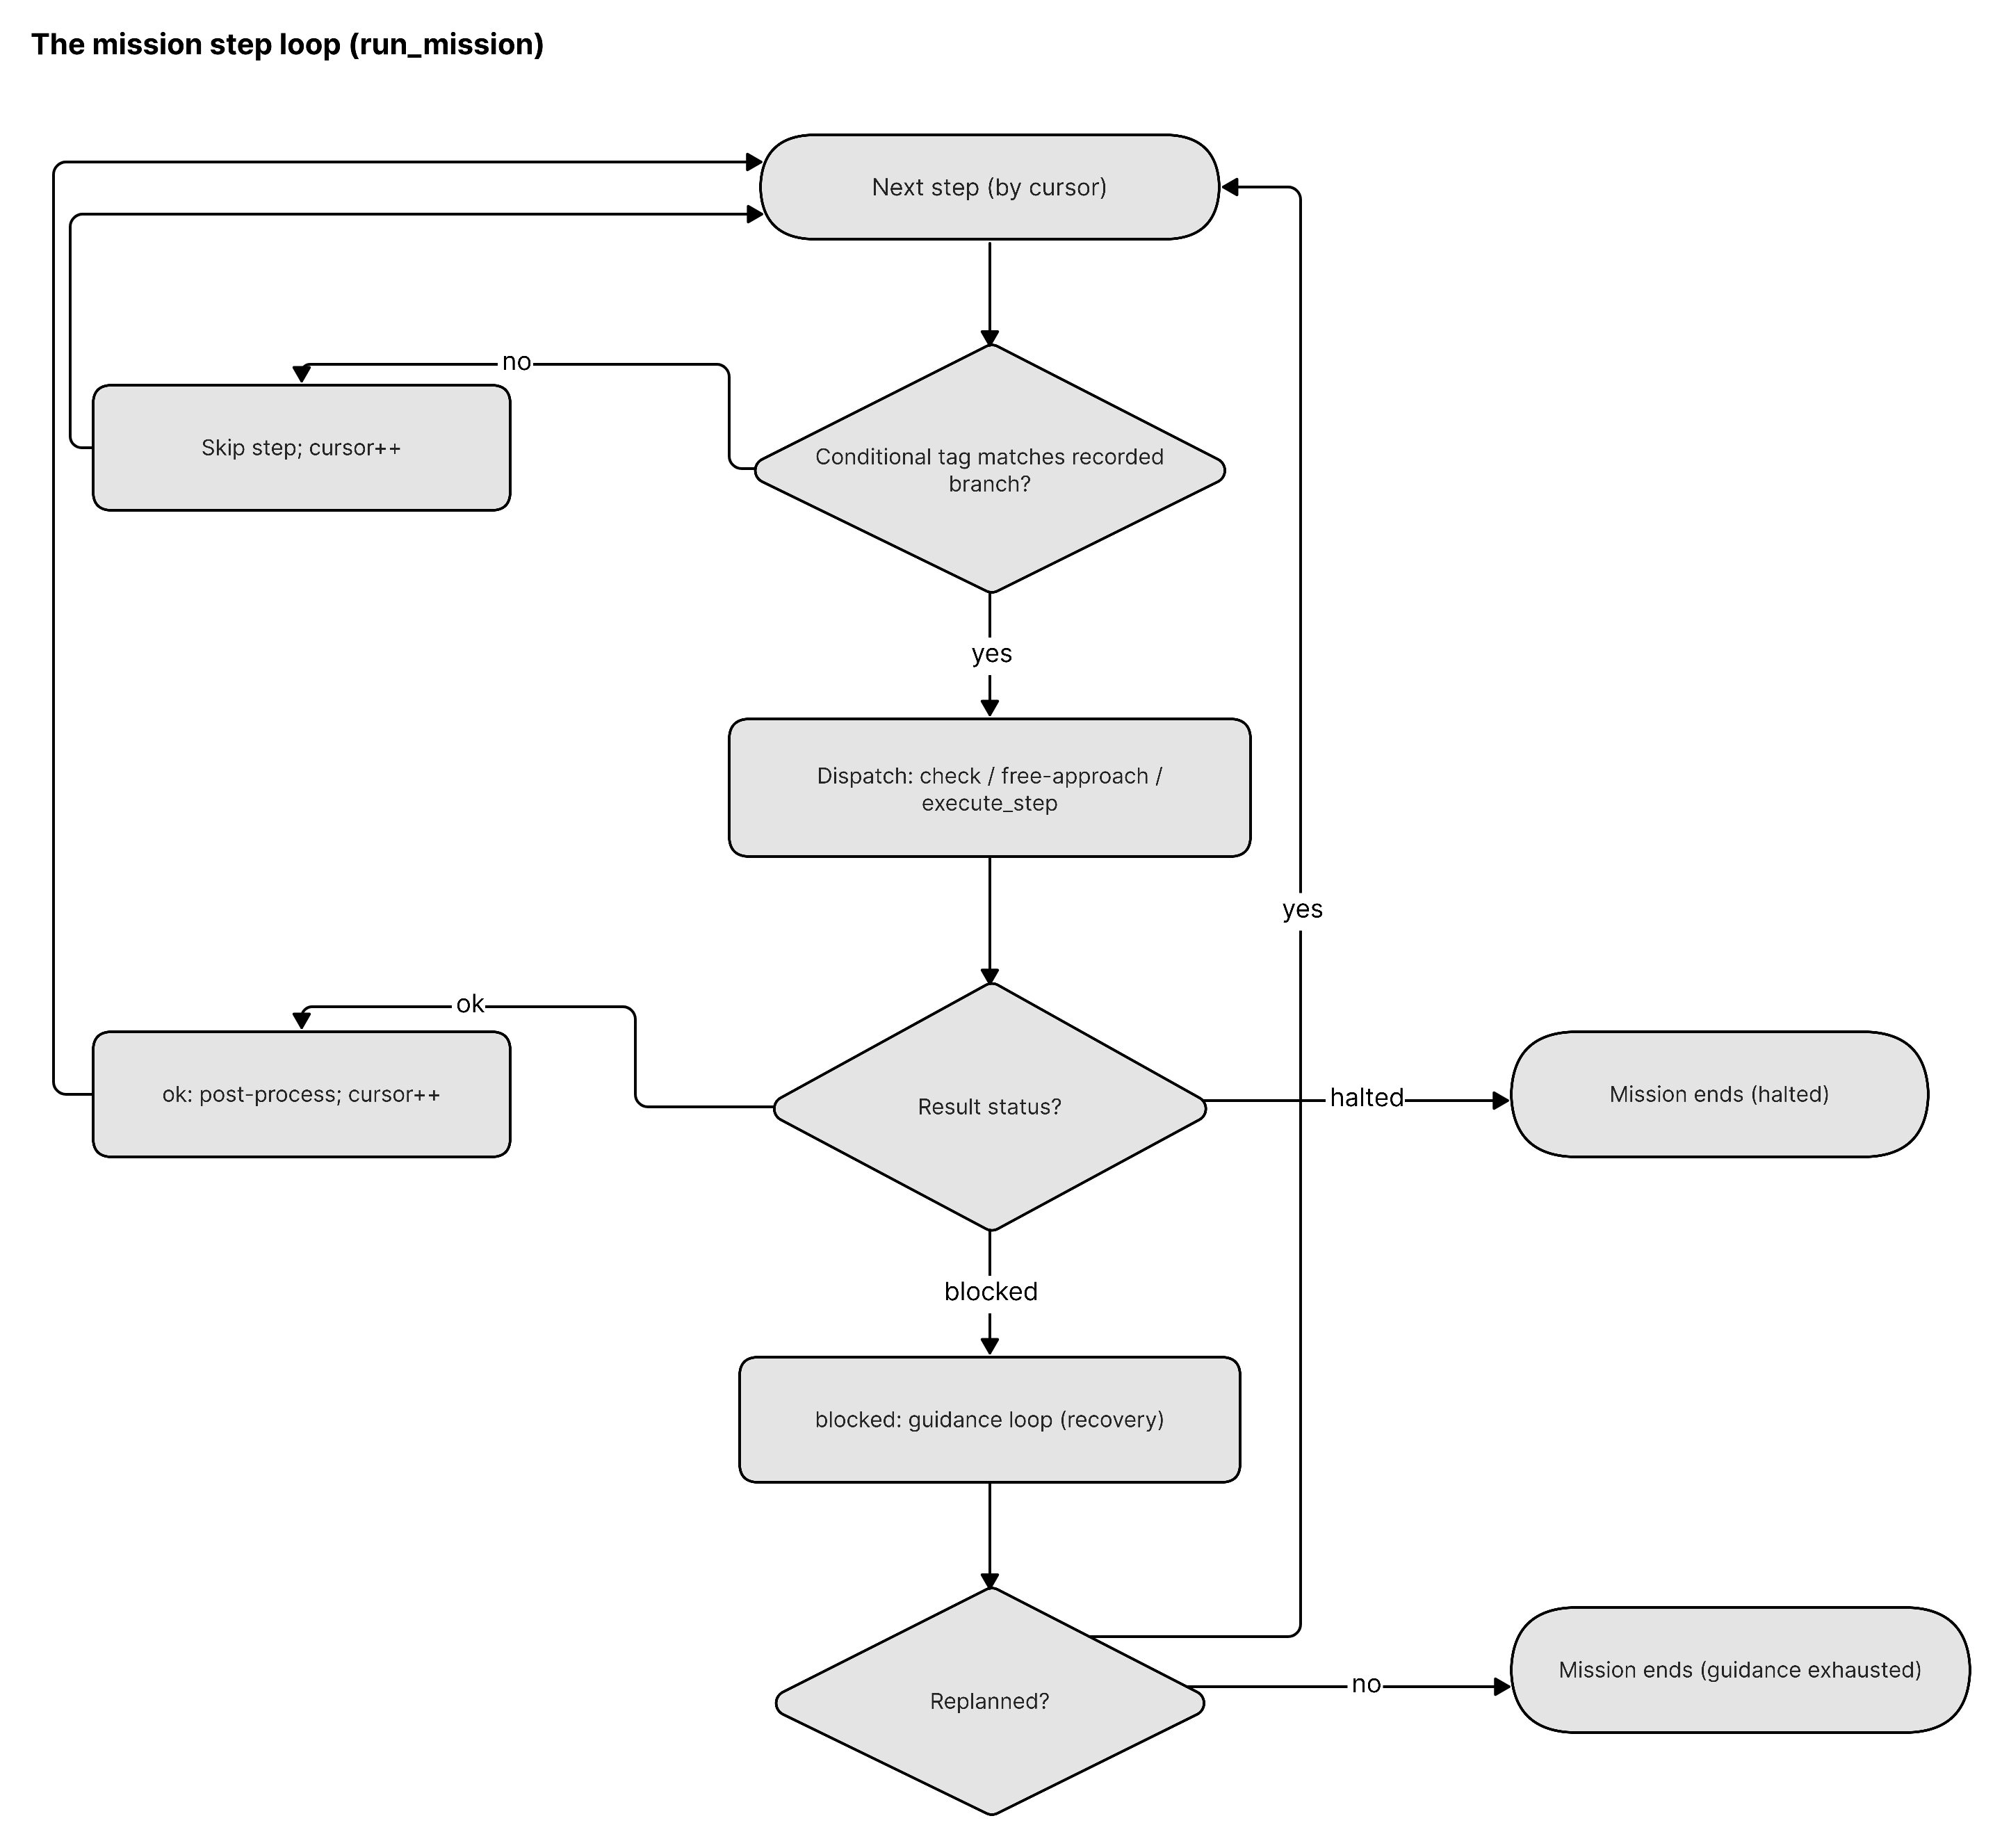
\includegraphics[width=\linewidth]{figures/fig_mission_loop.png}
  \caption{\texttt{run\_mission}'s step loop. The conditional-tag check is what Section~\ref{sec:conditional} relies on: the planner only decides which steps carry a \texttt{when} tag, and this check is what honours it. The loop's own \texttt{finally} block (not shown) writes the report for every non-aborted outcome; an operator-triggered \texttt{asyncio.CancelledError} skips straight to \texttt{rover.halt()} instead.}
  \label{fig:flow-mission}
\end{figure}

If a result is blocked it is handed off to the guidance loop (Section~\ref{ssec:guidance_loop}). A \texttt{halted} results
ends the mission immediately with no guidance offered, this comes down to the step itself deciding that the mission cannot continue. This
could be something in the way of the rover. If the mission was not aborted it will write  its report in the loop's \texttt{finally} block. It does 
not matter if it finished cleanly or ran out of guidance, or it was halted outright. All runs are tagged to be able to compare the results 
of why it was halted. The only path that skips writing an report is \texttt{asyncio.CancelledError}. It calls the \texttt{rover.halt()}
immediately and writes the determinitsitc half of the report straight to the disk with \texttt{spoken=False}, stopping the rover is never delayed
by a planner call or spoken summary. 

\mysubsection{Failure reovery in code}{Failure Recovery in Code}
\label{ssec:guidance_loop}

If the rover is \texttt{blocked} it is handed to \texttt{\_guidance\_loop}, which is the recovery behaviour of Section~\ref{sec:recovery} is 
implemented. The rover stops immediately if the \texttt{GUIDANCE\_ENABLED} flag is off. This is for testing purposes only. The guidance loop then
builds a question from a fixed template keyed on the failure reason  (\texttt{target\_not\_found}, \texttt{obstacle},
\texttt{arrival\_contradicted}, \texttt{cycle\_budget\_exhausted}, or a
generic fallback) and it asks the user up to 3 times on what its next steps are. The questions for guidance are templated and not generated
by a model for the simple fact that the model might have planned incorrectly so it is not a good idea to ask the source of the error why It
has stopped. This makes it predictable to know that the rover is lost and needs the actual steps to get to its target.

\begin{figure}[htbp]
  \centering
  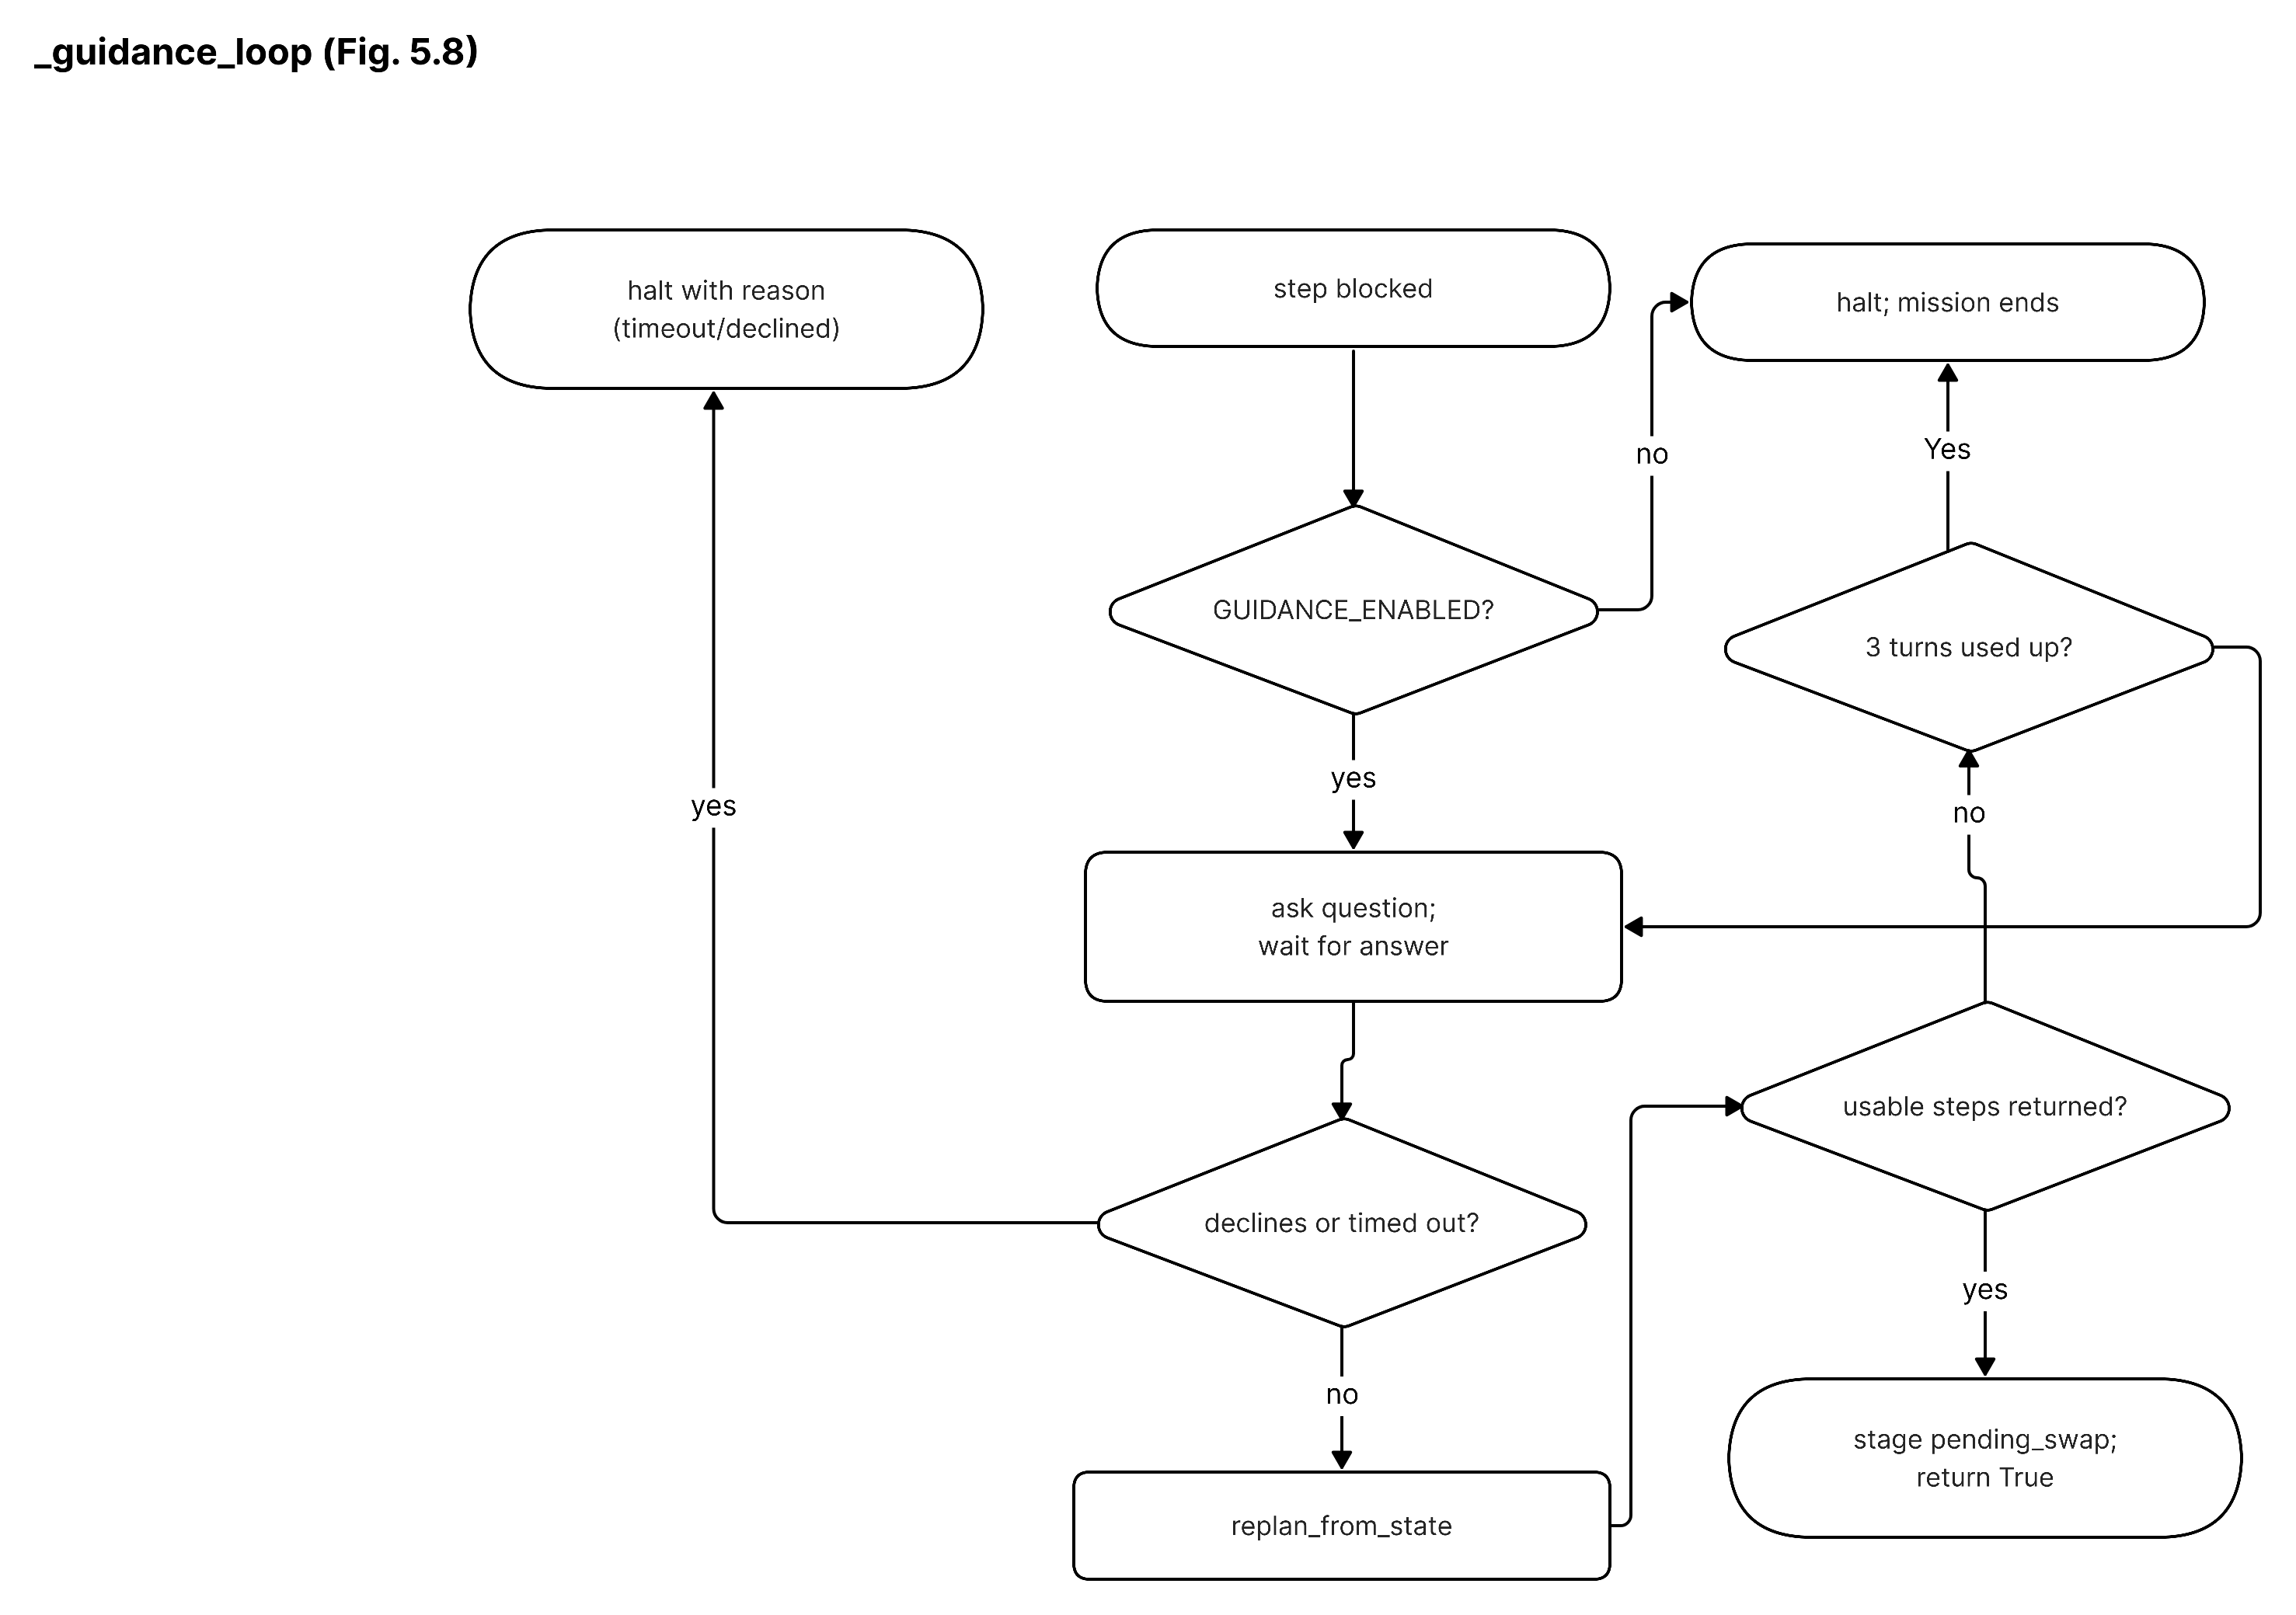
\includegraphics[width=\linewidth]{figures/fig5_8_flow_guidance.png}
  \caption{\texttt{\_guidance\_loop}. A ``no'' out of the turn-count check on the right loops back to ask again rather than ending the mission; running out of turns is itself a third halt reason (\texttt{guidance\_exhausted}), alongside timeout and decline, so a batch of failed runs can be told apart by why they failed.}
  \label{fig:flow-guidance}
\end{figure}

%====================postential section for _declines that needs to come in

\mysubsection{Mid-mission revision}{Mid-mission Revision}
\label{ssec:revision_impl}

The frames sent from the rover during a mission is sent through \texttt{ingest\_frame}, which has 3 checks to limit the amount of
calls to a bigger model. The VLM is not asked to look at every single frame. this is used since the rate at which the camera produces
frames is higher than the rate at which the VLM can process images. The three tiers in Figure~\ref{fig:flow-revision} let cheap, local checks
filter out the frames which are very similar and the VLM can prioritize the frames which are unique.


\begin{figure}[htbp]
  \centering
  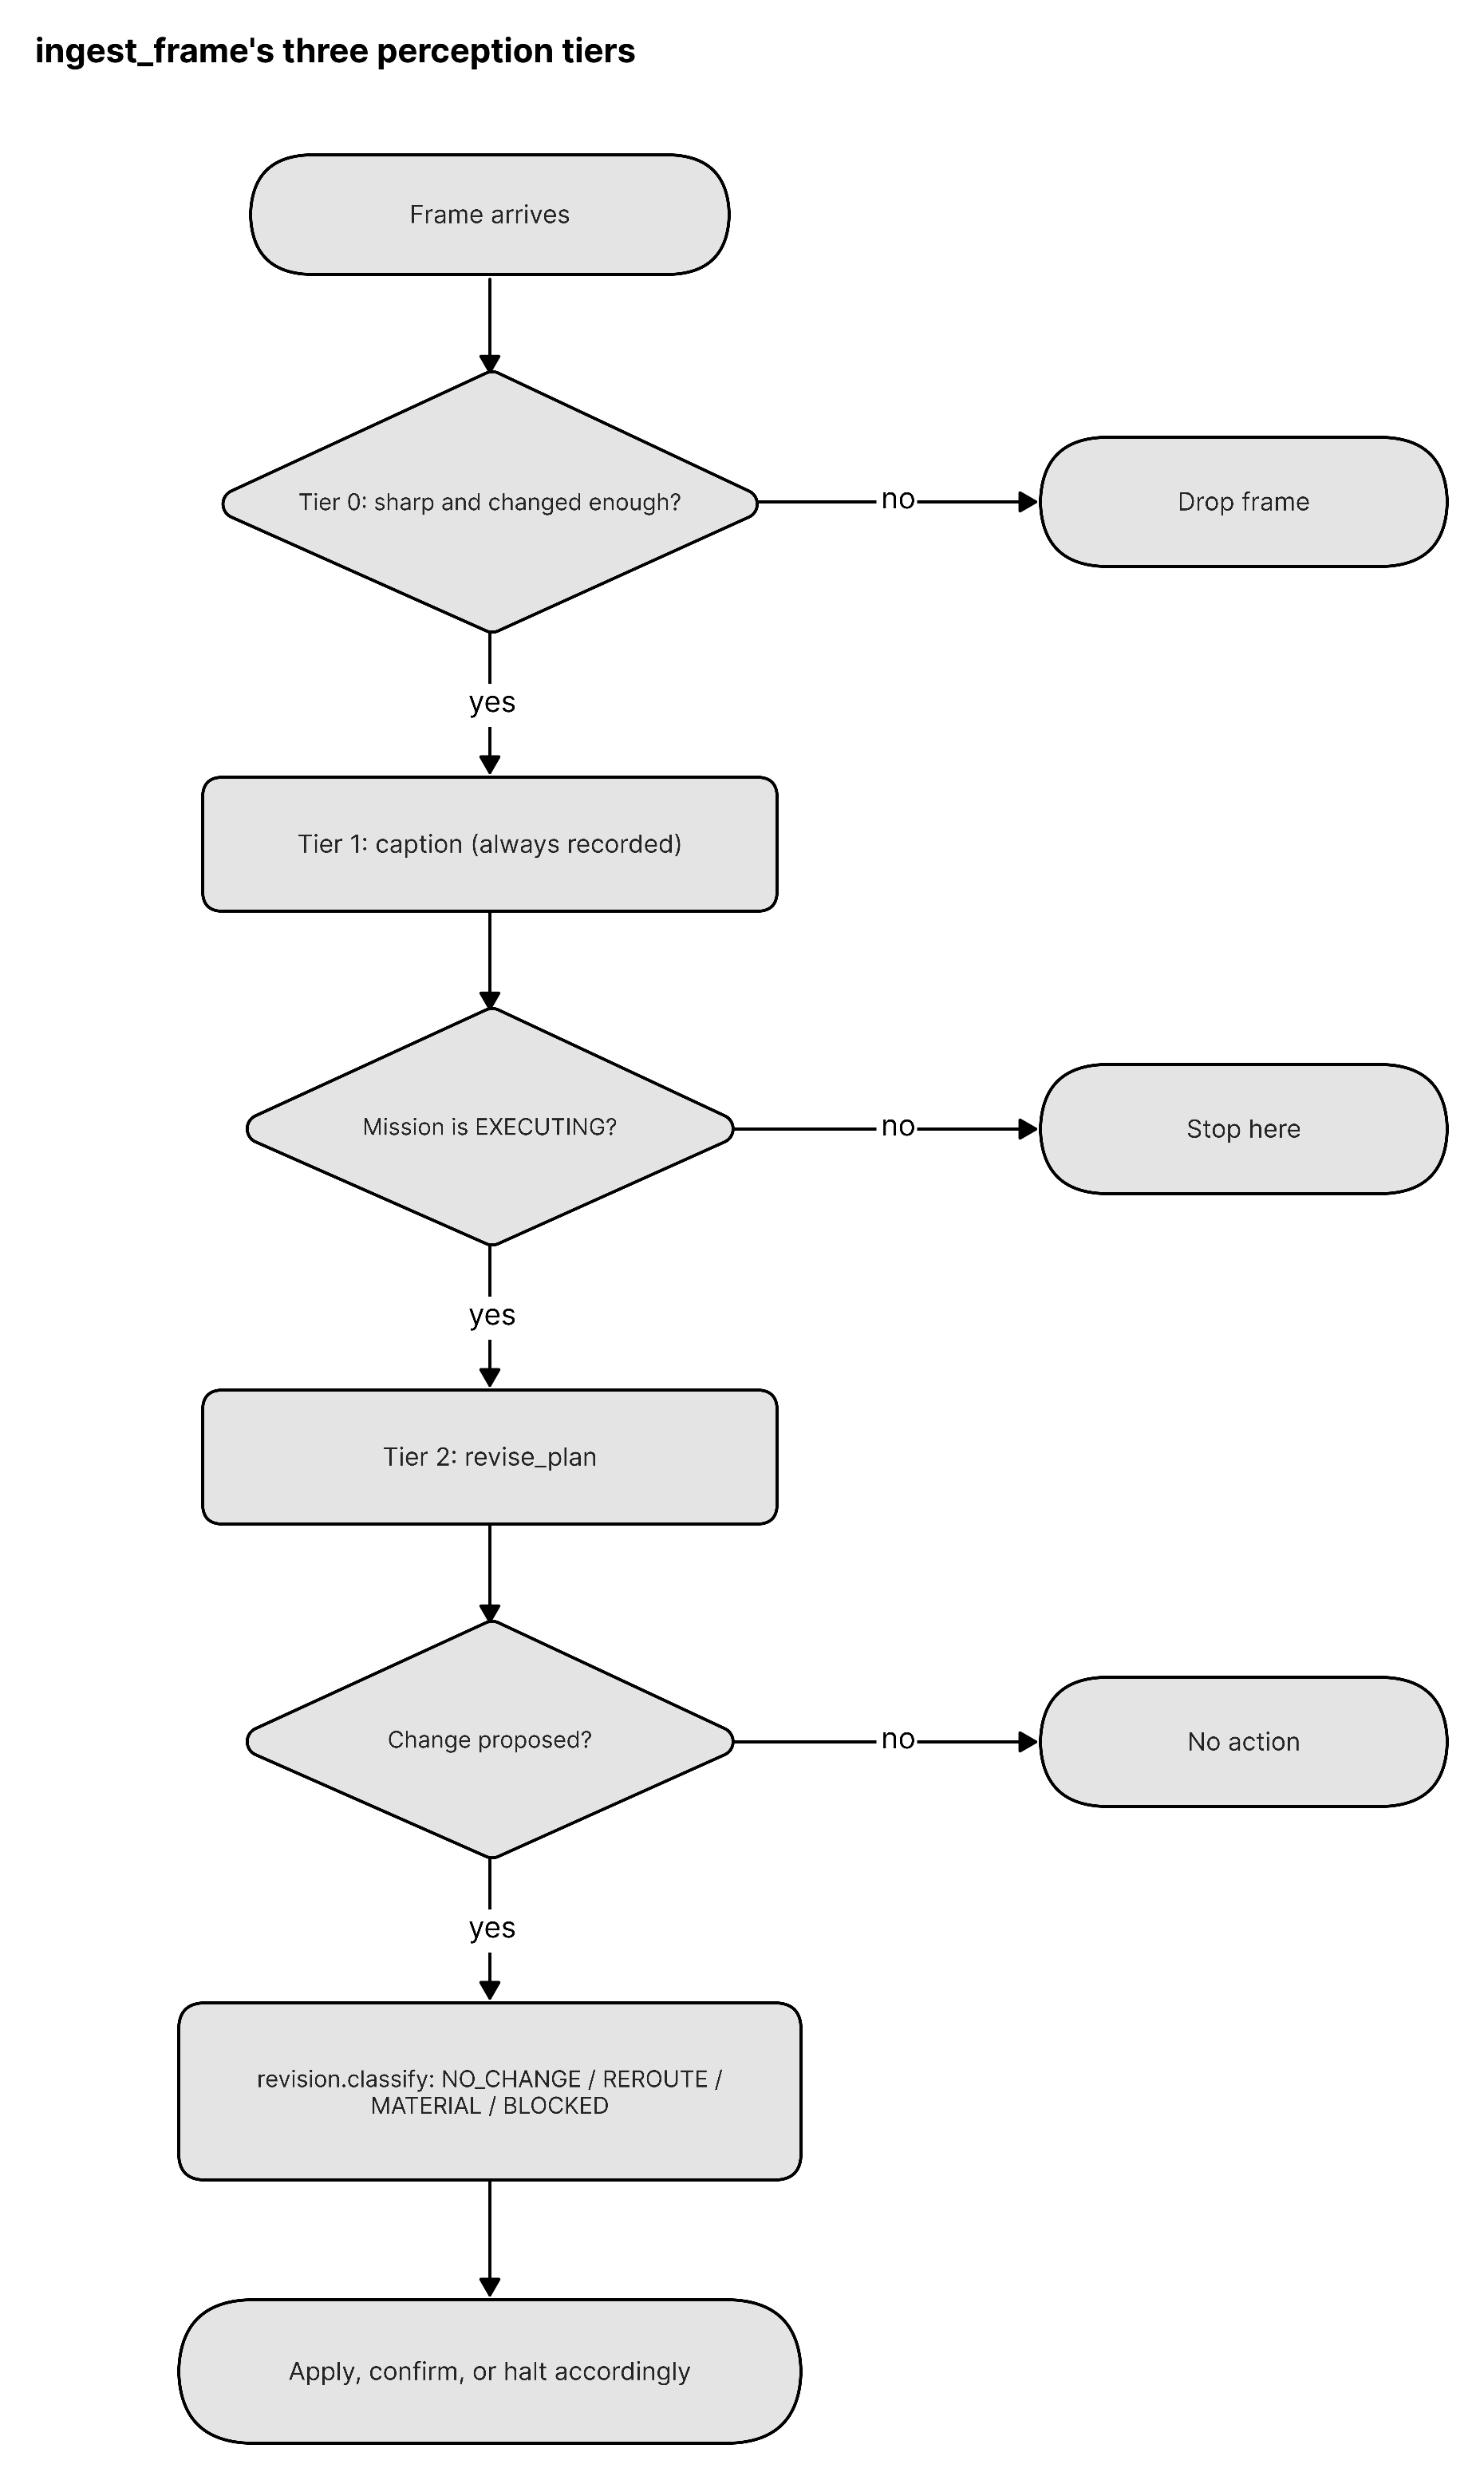
\includegraphics[width=\linewidth]{figures/fig_perception_tiers.png}
  \caption{\texttt{ingest\_frame}'s three tiers, feeding \texttt{revision.classify}. Tier 0 is a 32$\times$32 greyscale thumbnail diff plus a Laplacian-variance blur score (\texttt{PERCEPTION\_MIN\_SHARPNESS}, \texttt{PERCEPTION\_MIN\_INTERVAL\_S}, \texttt{PERCEPTION\_CHANGE\_THRESHOLD}); tier 1 is one \texttt{describe\_frame} caption; tier 2 only fires while executing.}
  \label{fig:flow-revision}
\end{figure}



The \texttt{revisioin.classify} is a plain rule, no model calls at all. It compares
the confirmed plan's targets against the proposed plan's. Using the action vocabulary for 
the specific rover. If you add a target, removing a confirmed target or a new action is introduced that is outside of the 
fixed navigation whitelist of tartgets. These all count as \texttt{MATERIAL} changes and stops the mission for a yes confirmation.
Then \texttt{handle\_revision\_confirmation} applies it. If there is an empty revised plan is \texttt{BLOCKED} it ends the mission as 
well since there is nothing to revise. If the goal and every target is unchanged, and the only new actions are navigation such as a different
route around an obstacle. This is treated as a small \texttt{REROUTE} that the rover can follow without confirmation.


\mysection{Rover client and reactive layer}{Rover Client and Reactive Layer}
\label{sec:rover_client}

\mysubsection{Real hardware: PiRoverController}{Real Hardware}
\label{ssec:pi_rover}


Inside of the \texttt{RoverController} is an abstract class with two required methods,
\texttt{execute\_step} and \texttt{halt}, as well as a optional \texttt{status\_light},
which is only available on rovers which have the status light hardware installed. 
This functionality is simple.  Every rover implementation has to run a step
and has to be able to stop. There are interfaces the physics-free simulator,
and a rover which communicates over ROS2 over a network socket. There are two main
rovers the \texttt{VirtualRover}, describe in Section~\ref{ssec:virtual_rover},
and \texttt{PiRoverController}, which controls the real TurboPi using roslibpy.

The \texttt{PiRoverController} opens one \texttt{roslibpy.Ros} connection,
advertises a \texttt{/cmd\_vel} topic for driving and a PWM-servo topic for the
gimbal. It also opents two ROS2 services to access \texttt{/line\_follow/cmd} and
\texttt{/line\_follow/set\_runnning}. These services control the stock line-follower
node rather than reimplementing line following from scratch. 



\begin{figure}[htbp]
  \centering
  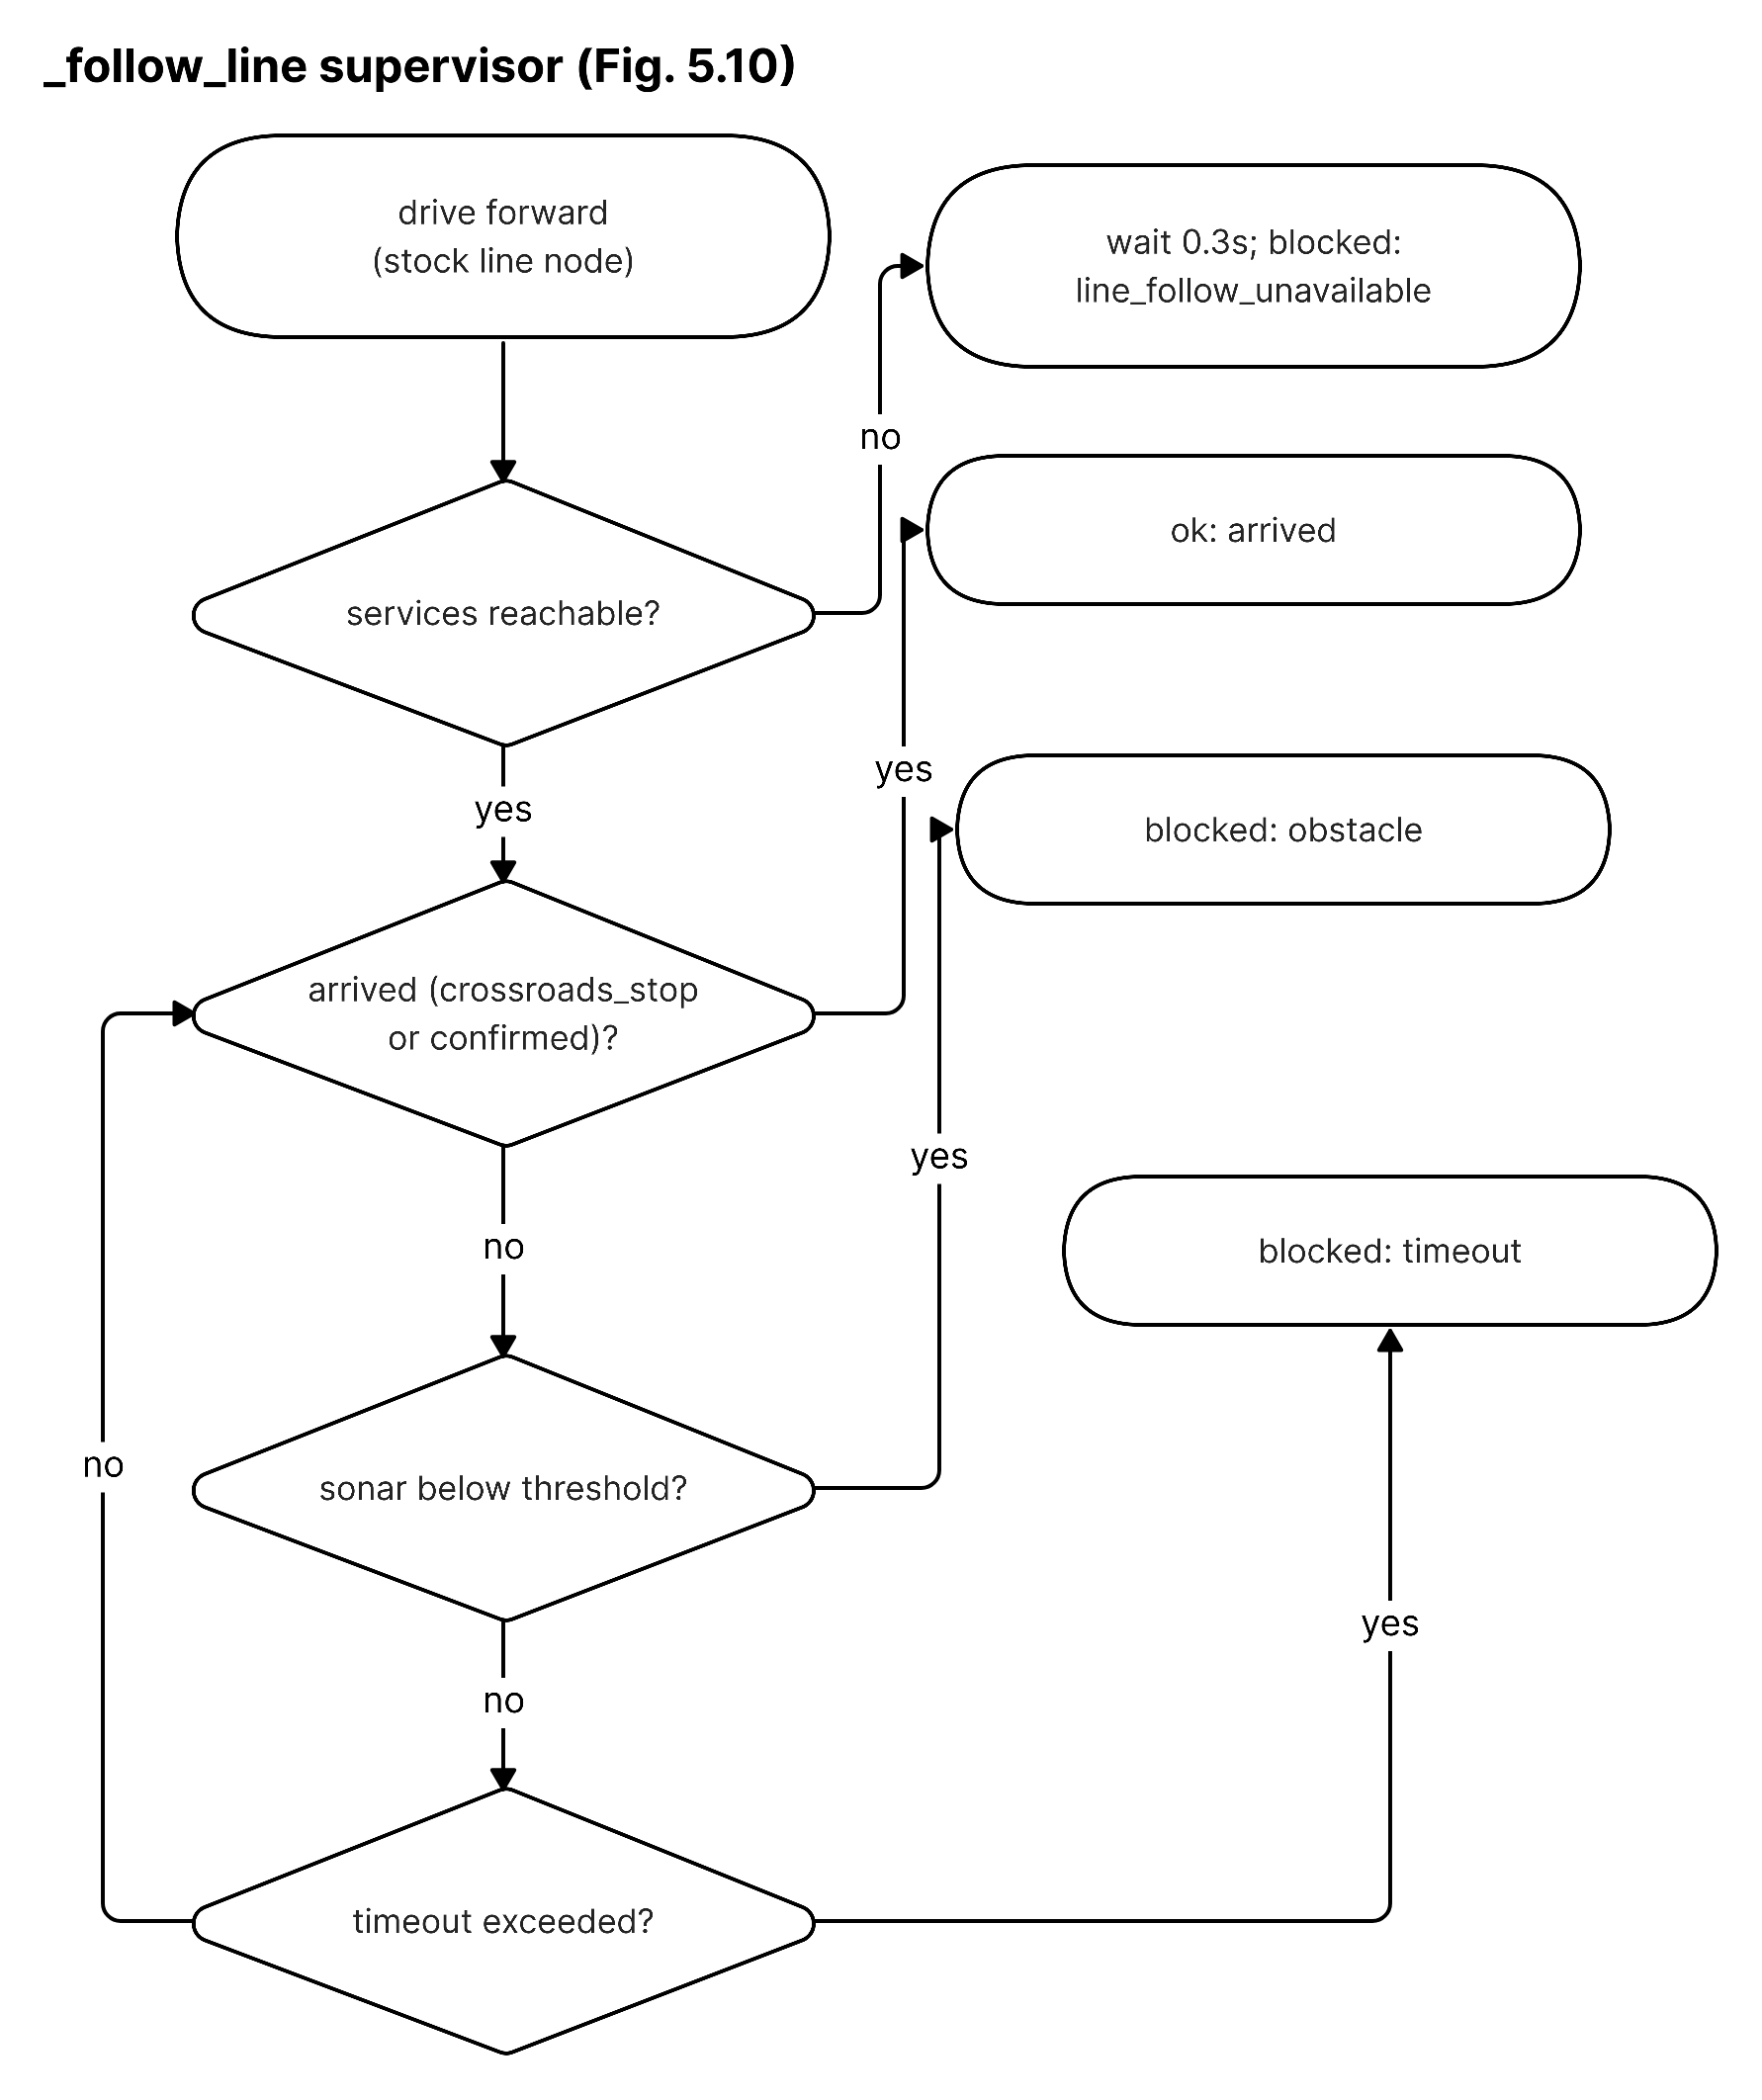
\includegraphics[width=\linewidth]{figures/fig5_10_flow_followline.png}
  \caption{\texttt{\_follow\_line}, the supervisor added around the stock line-follower node. It owns exactly the three things the node has no opinion about: arrival, obstacle stopping through the polled sonar (using \texttt{\_sonar\_seq} to tell two fresh readings from one stale one read twice), and a wall-clock give-up, since the node itself drives forward indefinitely if the line is lost. The \texttt{\_lf\_unavailable} check (added 11 October) means a drive that never started is reported as blocked rather than as a drive that ran and found nothing.}
  \label{fig:flow-followline}
\end{figure}


\mysubsubsection{Virtual testing: Virtual Rover}{Virtual Testing}
\label{ssec:virtual_rover}

This is where almost every piece of evaluation data comes from. the \texttt{VirtualRover} is what every
single run without physical hardware actually executes on. The virtual rover is built
around one idea: \texttt{approach} is a navigation skill, It plans a routes and follows
it, while the normal \texttt{move} and \texttt{turn} are commands which execute as give 
like drive forward, or turn right. The approach step hands over the target to the
rover and expects it to work out how to get there, while a \texttt{move} and \texttt{turn} step only 
hands over a specific distance or angle.

Both halves read from the same OccupancyGrid (nav.py), built once per room with the rover's footprint 
clearance baked in, so the planner and the collision checker can never silently disagree about what's free.

\begin{figure}[htbp]
  \centering
  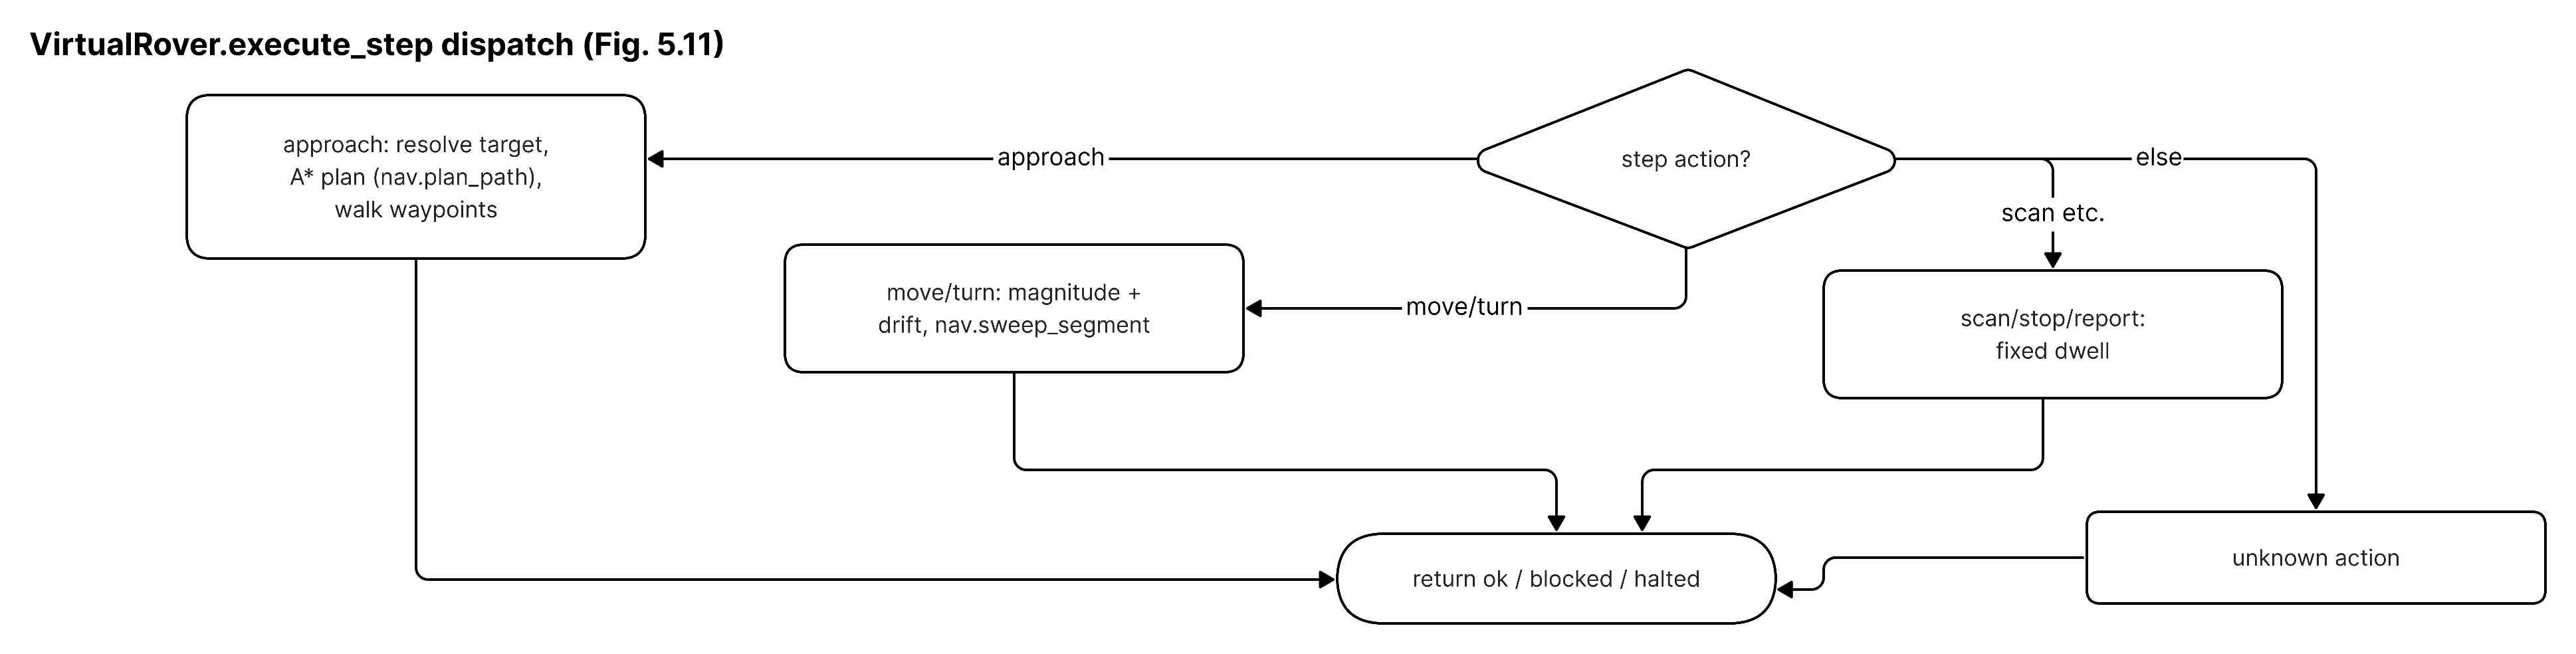
\includegraphics[width=\linewidth]{figures/fig5_11_flow_virtualrover.png}
  \caption{\texttt{VirtualRover.execute\_step}'s dispatch. An \texttt{approach} step can only fail by planning (no path, or an unresolved target logged as a hallucination for RQ2), never by collision; a \texttt{move} or \texttt{turn} step is swept against the same grid and stops at the last free point if blocked, so a collision there means the chain of plan steps itself went somewhere it should not have.}
  \label{fig:flow-virtualrover}
\end{figure}

The room itself, a \texttt{RoomMap} loaded from JSON
(\texttt{room\_map.py}), is hand-typed, not estimated. I measured
coordinates for every named landmark off a sketch and a tape measure once
per test room. A landmark's point is the standing spot a rover can occupy to look
at the thing. This is needed so the navigation code knows where the rover should end
up. The simulated and wall-clock time are kept apart the
same way: every action's duration is computed in simulated time first and
only then divided by \texttt{VIRTUAL\_TIME\_SCALE}. So a sweep of many runs
can be played back faster than real time without changing the distances,
speeds, or timings the evaluation actually reports on.

Every run writes one JSON line per step to a file to trace it and \texttt{summary()}
is able to derive statistics used for the second research question. Things like how many steps
counted, how many steps were blocked, how many targets were hallucinated and which ones. These
results are logged after each step rather than after the final outcome. Since a single 
pass/fail number does not contain the why it has that certain outcome.

\mysection{Communication protocol and dashboard}{Communication Protocol and Dashboard}
\label{sec:protocol}

The brain is a FastAPI application backend server. The two endpoints that matter for a
mission, \texttt{/ws/dialogue} and \texttt{/ws/execution}, are WebSockets
carrying small JSON frames rather than a request-response API, since both
sides need to push events the other did not ask for, the brain needs to
tell the Pi client a step started without the client polling for it, and
the client needs to tell the brain a frame arrived without the brain asking
for one on a timer. A request-response API would have meant one side
constantly polling the other for events that have no fixed schedule, which
is wasteful and adds latency. This is a
message protocol rather than a branching algorithm, so
Figure~\ref{fig:protocol} below is a sequence diagram, not a flowchart: it
shows who sends what, not a decision to be made.

\begin{figure}[htbp]
  \centering
  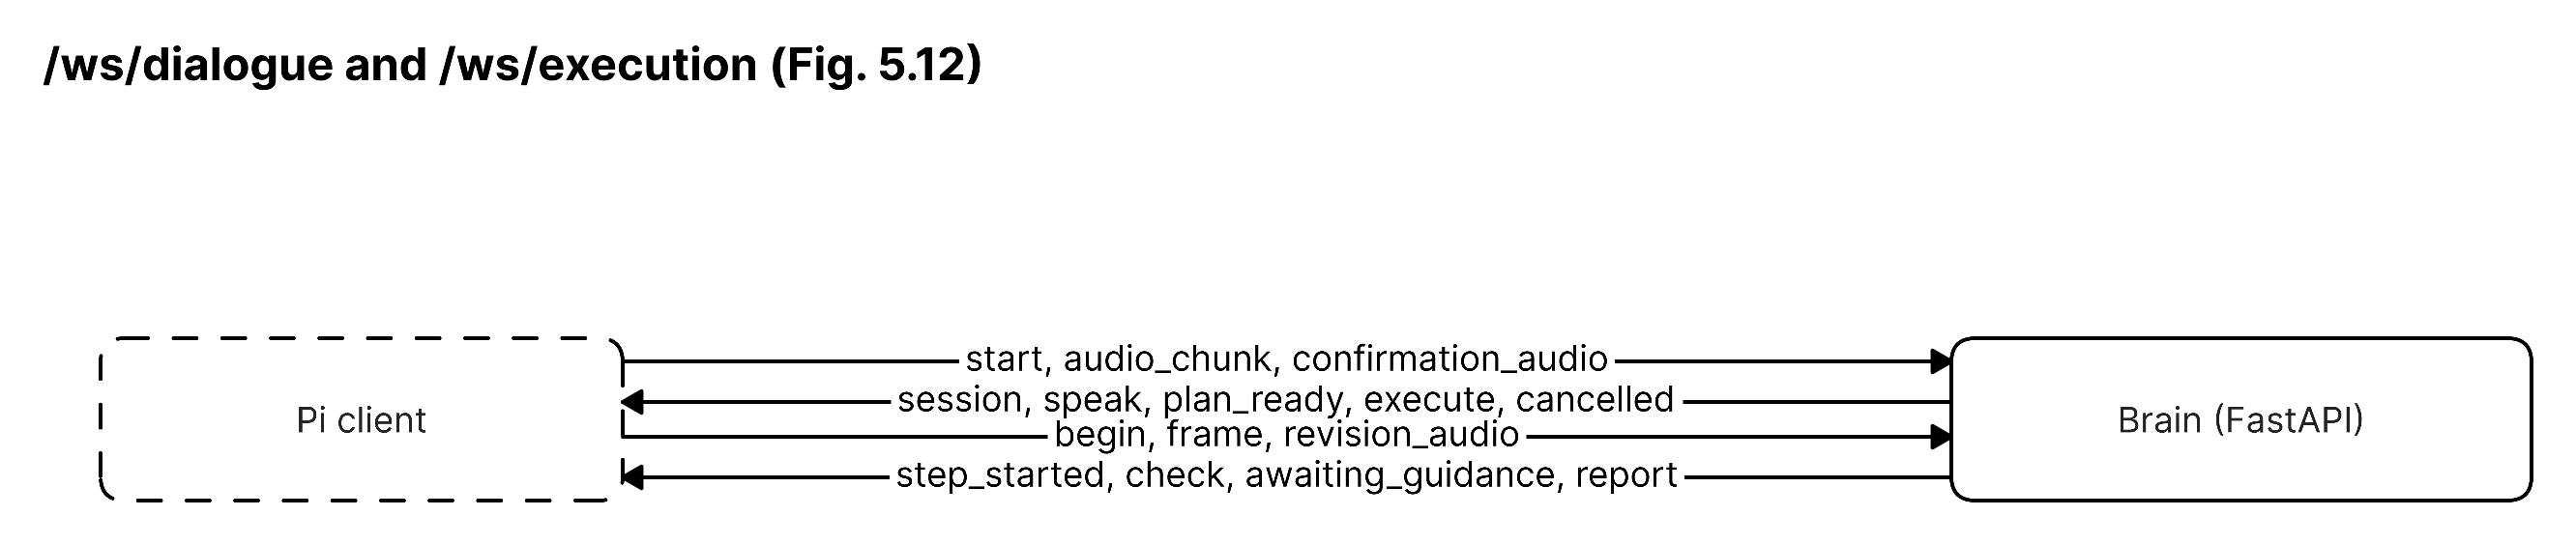
\includegraphics[width=\linewidth]{figures/fig5_12_protocol.png}
  \caption{\texttt{/ws/dialogue} (top pair) carries everything up to confirmation; \texttt{/ws/execution} (bottom pair) carries the mission. One frame per complete utterance, not a stream.}
  \label{fig:protocol}
\end{figure}

 Both connections are opened with \texttt{max\_size=None}. This was not the
original setting. A long spoken plan read-back,
a \texttt{speak} event carrying the base64 WAV Section~\ref{ssec:tts}
describes, exceeded the websockets library's 1\,MiB default size and closed the
connection. A few smaller endpoints round out the API. The \texttt{/scene} endpoint accepts an
uploaded walkthrough video and returns a scene id. The \texttt{/logs} endpoint and
\texttt{/logs/\{session\_id\}} endpoint serve the run log listing and detail that
the dashboard's Logs page reads from. There is a small \texttt{/logs/\{session\_id\}/flag}
endpoint that lets an operator mark a run good, bad
or for review with a note

The dashboard is a React and TypeScript single-page app, a thin client over
these same endpoints, and it holds no logic of its own that the evaluation
depends on, every number Chapter~\ref{chap:evaluation} reports comes from
the JSON logs, never from anything the UI computed on its own. It is a debugging and
demonstration tool and nothing more. Something that lets me upload a room
walkthrough video, watch a dialogue and a mission happen panel by panel,
and drive the rover manually, all without needing a terminal open

\mysection{Logging and measurement instrumentation}{Logging and Measurement Instrumentation}
\label{sec:logging}


There are two logging methods used here. The \texttt{brain.log} is a conventional application log, written
through Python's \texttt{logging} module,interleaving every call in time
order with full prompts and raw model output at debug level. Then we have the run log, one JSON file per executed mission.
This is the run log our evaluaiton secition gets the information it needs. The \texttt{report.py} file assembles: he plan, every check and its
result, the guidance log, the light-state timeline, the model tag for both
roles, and a tagged \texttt{test\_level} when one is set.

\begin{figure}[htbp]
  \centering
  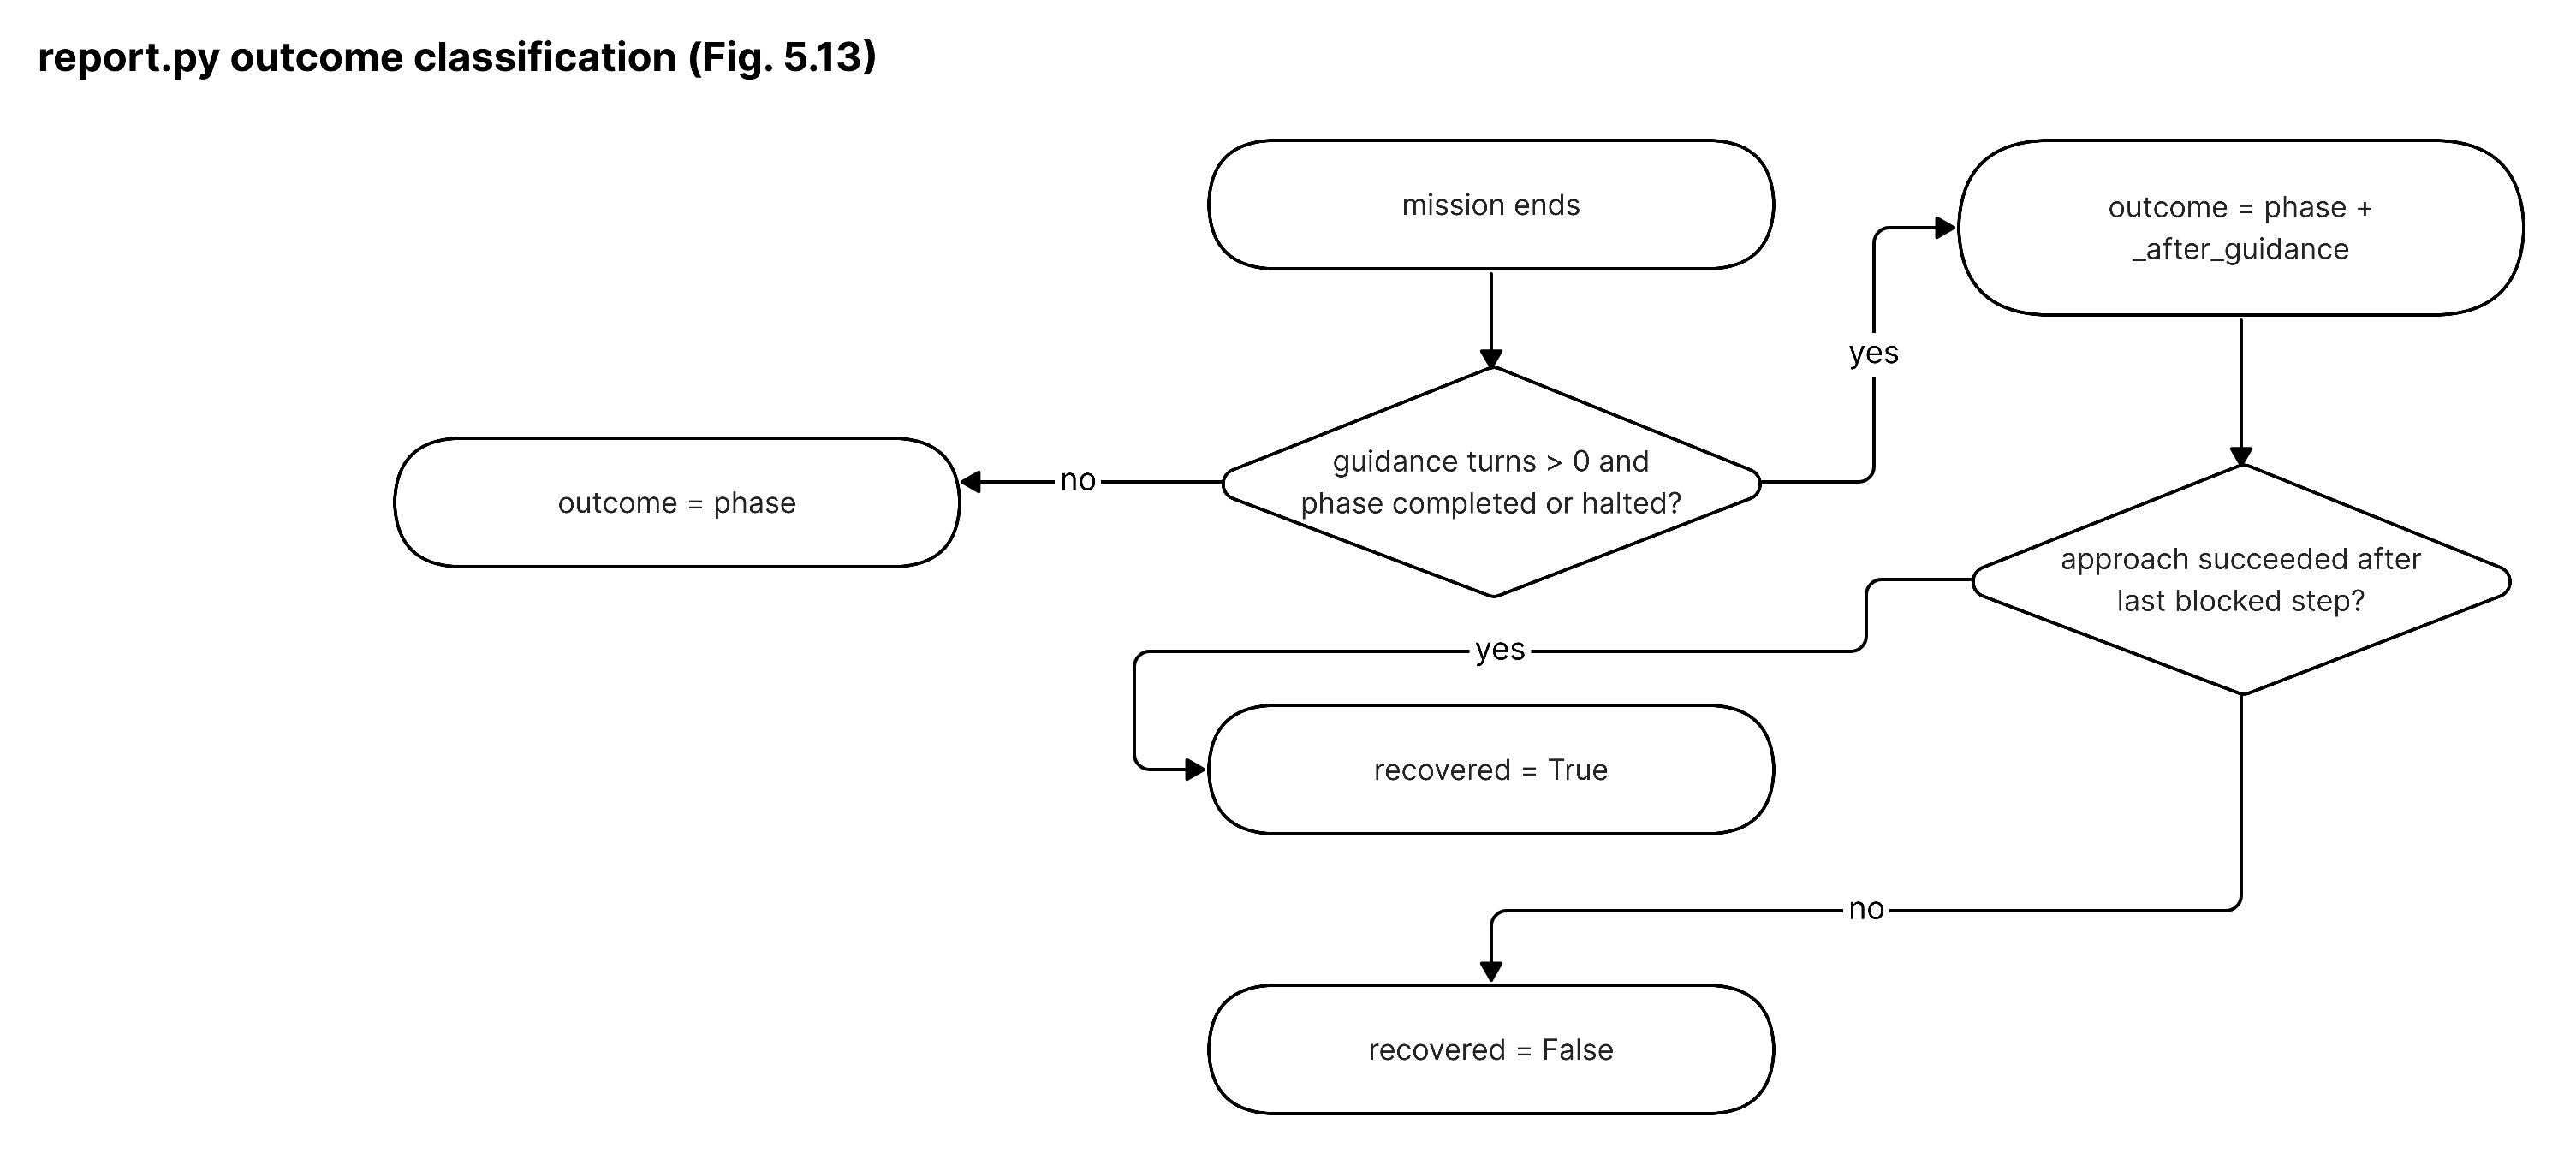
\includegraphics[width=\linewidth]{figures/fig5_13_flow_outcome.png}
  \caption{\texttt{report.py}'s outcome classification. A mission that needed at least one guidance turn is never reported as a plain \texttt{completed}, even if it finished, because the distinction between a clean run and a recovered one (Section~\ref{sec:recovery}) is exactly what RQ1 needs to see; \texttt{recovered} only counts a run that actually reached its target afterwards, not merely one that ended without halting.}
  \label{fig:flow-outcome}
\end{figure}

Every model call also writes one entry to a smaller usage ledger
(\texttt{providers/usage.py}), holding latency, token counts and cost when
the provider reports them, and this is reset at the start of every session.
A separate, offline tool, \texttt{tools/context\_budget.py}, measures something the run log on
its own cannot. How many tokens a given prompt would cost before it is
ever actually sent to a model. If you  ask ollama for the \texttt{prompt\_eval\_count} and send in a prompt with
the parameter \texttt{num\_predict=1}. It counts the tokens the
model would have to read without paying for a real generation afterward. It can measure the fixed instructions, t
he room digest, one clarification turn
and one recovery turn separately. This allows you to see a prompt's
token budget is actually going before running a mission to see if it would fail.